% ════════════════════════════════════════════════════════════════════════════
%  KDS-EL: Knowledge-guided Dual-Space Evolutionary Learning
%  for High-Dimensional Bioinformatics Feature Selection
%  Target: Expert Systems with Applications (ESWA)
% ════════════════════════════════════════════════════════════════════════════

\documentclass[a4paper,fleqn]{cas-dc}

\usepackage[authoryear]{natbib}
\usepackage{hyperref}
\usepackage{graphicx}
\usepackage{subfigure}
\usepackage{epstopdf}
\usepackage{color}
\usepackage[noend]{algpseudocode}
\usepackage{algorithmicx,algorithm}
\usepackage{amsmath,amssymb}
\usepackage{booktabs}
\usepackage{multirow}
\usepackage{bm}

%%% Author definitions
\def\tsc#1{\csdef{#1}{\textsc{\lowercase{#1}}\xspace}}
\tsc{KDS}
\tsc{DRS}
\tsc{KER}
\tsc{NHD}
\tsc{PSO}
%%%

\begin{document}
\begin{sloppypar}
	\let\WriteBookmarks\relax
	\def\floatpagepagefraction{1}
	\def\textpagefraction{.001}
	\let\printorcid\relax
	\shorttitle{KDS-EL for High-Dimensional Feature Selection}
	\shortauthors{Author et~al.}

	%% Title
	\title [mode = title]{Knowledge-guided Dual-Space Evolutionary Learning
	for High-Dimensional Bioinformatics Feature Selection}

	%% Authors -- replace with actual names and affiliations
	\author[1]{\textcolor[RGB]{0,0,1}{First Author}}
	\fnmark[1]
	\ead{first@university.edu.cn}

	\author[1]{\textcolor[RGB]{0,0,1}{Second Author}}
	\fnmark[1]
	\cormark[1]
	\ead{second@university.edu.cn}

	\author[1]{\textcolor[RGB]{0,0,1}{Third Author}}
	\fnmark[1]
	\ead{third@university.edu.cn}

	\address[1]{School of Computer Science and Technology, University Name, City, Country}

	\cortext[cor1]{Corresponding author.}
	\fntext[fn1]{Equal Contribution.}

	%% Highlights
	\begin{highlights}
	\item Propose a bi-objective-regulated dual-space evolutionary learning
	      framework (KDS-EL) for high-dimensional bioinformatics feature selection.
	\item Design a Diversity-regulated Selection (DRS) operator that elevates
	      NHD into a first-class Pareto selection objective to prevent structural collapse.
	\item Develop a Knowledge-guided Elite Refinement (KER) mechanism that
	      accumulates improvement evidence online to direct targeted bit-flip perturbations.
	\item Demonstrate synergistic gain of DRS and KER on 7 of 9 benchmark datasets.
	\item Achieve superior classification accuracy and maximum feature reduction
	      against eight competitors including PSO-CSM (2025) and IGPSO (2024).
	\end{highlights}

	%% Abstract
	\begin{abstract}
	Feature selection is essential for reducing dimensionality and improving
	classifier performance in high-dimensional bioinformatics data, where
	the exponential search space makes evolutionary methods highly
	susceptible to structural population collapse and knowledge waste.
	To address these coupled challenges, we propose \textbf{KDS-EL}
	(\textit{Knowledge-guided Dual-Space Evolutionary Learning}), a novel
	bi-objective-regulated evolutionary framework that simultaneously
	optimises a dual-population PSO backbone across two complementary
	search spaces.
	First, we design a \textbf{Diversity-regulated Selection} (DRS) operator
	that elevates Normalised Hamming Distance (NHD) from a post-hoc
	diagnostic metric to a first-class Pareto selection objective,
	providing a provable structural diversity lower bound and preventing
	premature population convergence.
	Second, we develop a \textbf{Knowledge-guided Elite Refinement} (KER)
	mechanism that accumulates improvement-event evidence from the
	evolutionary trajectory into a feature-importance weight vector,
	and uses this online-learned knowledge to direct targeted bit-flip
	perturbations of elite solutions without additional fitness evaluations.
	The two mechanisms are synergistically coupled: DRS's structural
	diversity ensures heterogeneous improvement signals for KER, while KER's
	directed perturbations enrich the DRS selection pool.
	Extensive experiments on nine high-dimensional bioinformatics datasets
	($d \in [927,\,26{,}877]$) against eight state-of-the-art competitors
	demonstrate that KDS-EL achieves the highest average Friedman rank
	of 1.222 (Friedman $\chi^2=47.38$, $p=1.30\times10^{-7}$),
	reduces selected feature counts by up to 88\% relative to the base
	framework, and outperforms recent methods including PSO-CSM (2025)
	and IGPSO (2024) across all nine datasets with statistical significance.
	Ablation analysis confirms positive synergistic gain on 7 of 9 datasets,
	validating the Dual-Space design rationale.
	\end{abstract}

	%% Keywords
	\begin{keywords}
		Feature selection \sep
		Evolutionary computation \sep
		Population diversity \sep
		Knowledge-guided learning \sep
		Bioinformatics
	\end{keywords}

	\maketitle

	% ════════════════════════════════════════════════════════════════════════
	%  1. INTRODUCTION
	% ════════════════════════════════════════════════════════════════════════

	\section{Introduction}
	\label{sec:intro}

	\par{
	With the rapid advances in high-throughput sequencing technologies,
	gene expression and other omics datasets routinely comprise tens of
	thousands of features measured over fewer than 200 samples
	\citep{bolnick2014precision,hampton2004introduction}.
	This extreme $d \gg n$ regime---where the number of features $d$
	exceeds the number of samples $n$ by orders of magnitude---poses
	severe challenges for classification algorithms, including the curse
	of dimensionality, overfitting, and prohibitive computational cost.
	Feature selection (FS), which identifies a compact and informative
	subset of the original features, has emerged as an indispensable
	preprocessing step in bioinformatics pipelines
	\citep{saeys2007review,dash1997feature}.
	Among FS paradigms, wrapper-based evolutionary methods that employ
	metaheuristic search---particularly Particle Swarm Optimisation
	(PSO)---have demonstrated strong empirical performance owing to
	their ability to explore the combinatorial binary search space
	without requiring differentiable objectives
	\citep{xue2015survey,wang2021particle}.
	}

	\par{
	Despite these advances, existing evolutionary FS methods suffer from
	two fundamental and coupled limitations.
	\textit{First}, most methods treat classification accuracy (or its
	surrogate fitness) as the sole selection criterion
	\citep{chuang2011binary,zhang2015adaptive,huang2020enhanced},
	leaving the \emph{structural geometry} of the binary solution space
	unexploited.
	In the high-dimensional binary landscape, random feature subsets
	exhibit low Normalised Hamming Distance (NHD) to one another;
	when combined with accuracy-only selection, this structural
	homogeneity drives rapid population collapse into a small region
	of the search space, prematurely eliminating potentially valuable
	feature combinations.
	To date, NHD has been used only as a post-hoc diversity diagnostic,
	never as a first-class selection objective within wrapper-based
	evolutionary FS.
	\textit{Second}, the cumulative evidence of which feature transitions
	proved beneficial during the search---the \emph{trajectory knowledge}---is
	discarded at every generation.
	Each time the personal best ($P_{\mathrm{best}}$) is updated,
	the information about which features contributed to the improvement
	is lost, wasting a valuable signal that could guide future search.
	}

	\par{
	To address these coupled challenges, we propose \textbf{KDS-EL}
	(\textit{Knowledge-guided Dual-Space Evolutionary Learning}),
	a bi-objective-regulated evolutionary framework that operates
	simultaneously in two complementary search spaces:
	(i)~a \emph{Structural Space}, where a Diversity-regulated Selection
	(DRS) operator elevates NHD to a first-class Pareto selection
	objective; and
	(ii)~a \emph{Fitness Space}, where a Knowledge-guided Elite
	Refinement (KER) mechanism accumulates improvement evidence from
	the evolutionary trajectory to direct targeted bit-flip
	perturbations of elite solutions.
	The two mechanisms are synergistically coupled: DRS maintains
	structural diversity in the population, ensuring that KER receives
	heterogeneous improvement signals; conversely, KER's directed
	perturbations generate high-quality diverse candidates that enrich
	the DRS selection pool.
	This synergy is the central design principle of KDS-EL and is
	empirically validated on 7 of 9 benchmark datasets.
	}

	\par{
	The main contributions of this paper are as follows:
	\begin{enumerate}[(i)]
		\item We propose KDS-EL, a dual-space evolutionary learning
		framework for high-dimensional bioinformatics feature selection
		that simultaneously optimises fitness and structural diversity.
		\item We design the DRS operator that incorporates NHD as a
		first-class Pareto selection objective, with a provable diversity
		lower bound and an adaptive schedule $\alpha_{\mathrm{cd}}(t)=(t/T)^2$
		that transitions smoothly from diversity exploration to accuracy
		exploitation.
		\item We develop the KER mechanism that accumulates
		improvement-event evidence into a feature-importance weight
		vector online, enabling directed elite refinement with no
		additional fitness evaluations and a single interpretable
		parameter.
		\item Extensive experiments on nine bioinformatics datasets
		against eight competitors---including PSO-CSM~(2025) and
		IGPSO~(2024)---demonstrate that KDS-EL achieves the highest
		average Friedman rank of 1.222, with statistical significance
		confirmed by Wilcoxon signed-rank tests.
	\end{enumerate}
	}

	\par{
	The remainder of this paper is organised as follows.
	Section~\ref{sec:related} reviews related work on evolutionary
	feature selection, population diversity maintenance, and
	knowledge-guided methods.
	Section~\ref{sec:method} presents the proposed KDS-EL framework
	in detail, including the DRS and KER mechanisms with their
	theoretical properties.
	Section~\ref{sec:experiments} reports the experimental setup,
	results, and discussion.
	Section~\ref{sec:conclusion} concludes the paper and outlines
	future research directions.
	}

	% ════════════════════════════════════════════════════════════════════════
	%  2. RELATED WORK
	% ════════════════════════════════════════════════════════════════════════

	\section{Related Work}
	\label{sec:related}

	\subsection{Evolutionary Feature Selection}
	\label{sec:related:evofs}

	\par{
	Feature selection methods can be broadly categorised into filter,
	wrapper, and embedded approaches~\citep{guyon2003introduction}.
	Wrapper methods evaluate candidate feature subsets by training and
	testing a classifier, making them more accurate but computationally
	more expensive than filter methods.
	Evolutionary computation (EC) techniques have been widely adopted
	as wrapper-based FS solvers due to their ability to navigate the
	$2^d$ combinatorial search space without requiring gradient
	information.
	Binary PSO (BPSO)~\citep{kennedy1997discrete} was among the first
	to adapt PSO for discrete optimisation, encoding feature subsets as
	binary vectors and using sigmoid transfer functions for position
	updates.
	Subsequent variants have improved upon BPSO in various directions.
	Adaptive inertia weight strategies have been proposed to balance
	exploration and exploitation across the search
	trajectory~\citep{zhang2015adaptive}.
	FWPSO~\citep{huang2020enhanced} introduces a feature-weight-based
	initialisation mechanism that accelerates convergence by biasing
	the initial population toward promising regions.
	SaWDE~\citep{zhan2020sa} combines self-adaptive differential
	selection with PSO, achieving competitive performance with reduced
	parameter tuning.
	MEL~\citep{MEL_CITE} proposes a dual-subpopulation architecture
	where one subpopulation performs standard PSO exploration while the
	other employs knowledge-guided sampling, demonstrating strong
	results on bioinformatics benchmarks.
	More recently, PSO-CSM~(2025) introduces a comprehensive scoring
	metric that integrates multiple criteria, and IGPSO~(2024)
	pre-trains a multi-layer perceptron (MLP) to estimate feature
	importance prior to the search.
	Despite these advances, the majority of existing methods treat
	classification accuracy as the sole selection objective, neglecting
	the structural information embedded in the binary solution space.
	Table~\ref{tab:literature} summarises the key characteristics of
	recent PSO-based FS methods.
	}

	\begin{table*}[t]
	\centering
	\caption{Summary of recent PSO-based feature selection methods.
	Div.~= diversity maintenance mechanism; Know.~= knowledge-guided mechanism.}
	\label{tab:literature}
	\setlength{\tabcolsep}{3pt}
	\begin{tabular}{lclccc}
	\toprule
	\textbf{Algorithm} & \textbf{Year} & \textbf{Reference} & \textbf{High-dim} & \textbf{Div.} & \textbf{Know.} \\
	\midrule
	BPSO     & 2011 & \citep{chuang2011binary}          & \checkmark & -- & -- \\
	SaWDE    & 2020 & \citep{zhan2020sa}                & \checkmark & -- & -- \\
	FWPSO    & 2020 & \citep{huang2020enhanced}         & \checkmark & -- & Initialisation bias \\
	MEL      & --   & \citep{MEL_CITE}                  & \checkmark & Dual subpop. & Weight feedback \\
	IGPSO    & 2024 & \citep{IGPSO_CITE}                & \checkmark & -- & MLP pre-training \\
	PSO-CSM  & 2025 & \citep{PSOCSM_CITE}               & \checkmark & -- & Scoring metric \\
	\textbf{KDS-EL} & -- & \textbf{This work}            & \checkmark & NHD Pareto & Improvement feedback \\
	\bottomrule
	\end{tabular}
	\end{table*}


	\subsection{Population Diversity in Evolutionary Feature Selection}
	\label{sec:related:diversity}

	\par{
	Population diversity is widely recognised as a critical factor
	affecting the performance of evolutionary algorithms, as insufficient
	diversity leads to premature convergence while excessive diversity
	slow convergence~\citep{morrison2002measurement,ursem2002diversity}.
	In the context of binary feature selection, diversity can be
	quantified by the Normalised Hamming Distance (NHD), which measures
	the proportion of differing feature inclusions between two solutions.
	Several diversity maintenance strategies have been proposed in the
	evolutionary FS literature.
	Multi-population approaches~\citep{MEL_CITE} split the swarm into
	subpopulations that explore different regions of the search space.
	Population reinitialisation methods periodically replace converged
	individuals with random solutions to restore
	diversity~\citep{ursem2002diversity}.
	Crowding and sharing techniques, originally proposed for
	multi-objective optimisation~\citep{deb2002fast}, have been adapted
	to maintain diversity in FS populations.
	However, these approaches treat diversity as a secondary concern---a
	means to avoid stagnation rather than a formal optimisation target.
	To the best of our knowledge, KDS-EL is the first wrapper-based
	evolutionary FS method to incorporate NHD as a first-class Pareto
	selection objective within a bi-objective selection framework,
	providing a provable diversity lower bound rather than an ad-hoc
	maintenance heuristic.
	}


	\subsection{Knowledge-Guided and Multi-Task Evolutionary FS}
	\label{sec:related:knowledge}

	\par{
	Knowledge-guided evolutionary algorithms aim to leverage information
	accumulated during the search process to improve efficiency and
	solution quality~\citep{jin2011surrogate}.
	In the FS domain, IGPSO~\citep{IGPSO_CITE} pre-trains an MLP on
	a subset of the data to estimate feature importance, incurring a
	one-time training cost of $\Phi = O(d \cdot h \cdot \text{epoch})$
	where $h$ is the hidden layer size.
	While effective, this approach requires dataset-specific
	hyperparameter tuning and cannot adapt to the evolving search
	landscape.
	FWPSO~\citep{huang2020enhanced} uses feature weights for
	initialisation but does not update these weights during the search,
	discarding the trajectory knowledge.
	SAR-MTPSO~\citep{SARMTPSO_CITE} constructs a multi-task framework
	with heterogeneous fitness functions (compactness-focused and
	accuracy-focused), exploiting objective heterogeneity for knowledge
	transfer across tasks.
	However, SAR-MTPSO solves a fundamentally different problem---it
	decomposes a single objective into multiple tasks---and its
	architecture is not directly comparable to single-objective
	formulations such as KDS-EL.
	PSO-CSM~(2025) introduces a comprehensive scoring metric that
	integrates classification accuracy with feature count, but does
	not incorporate structural diversity or trajectory knowledge.
	In contrast, KDS-EL's KER mechanism accumulates improvement-event
	evidence from the evolutionary trajectory into a feature-importance
	weight vector \emph{online}, without any pre-training or additional
	fitness evaluations, and uses a single interpretable parameter
	(random flip probability $p_r$) to guarantee ergodicity.
	}

	% ════════════════════════════════════════════════════════════════════════
	%  3. METHODOLOGY
	% ════════════════════════════════════════════════════════════════════════

	\section{The Proposed KDS-EL Framework}
	\label{sec:method}

	Figure~\ref{fig:framework} illustrates the overall architecture of
	KDS-EL, which operates simultaneously in two complementary search
	spaces: the \emph{Structural Space} (DRS) and the \emph{Fitness
	Space} (KER). The following subsections detail each component.

	\begin{figure*}[t]
	\centering
	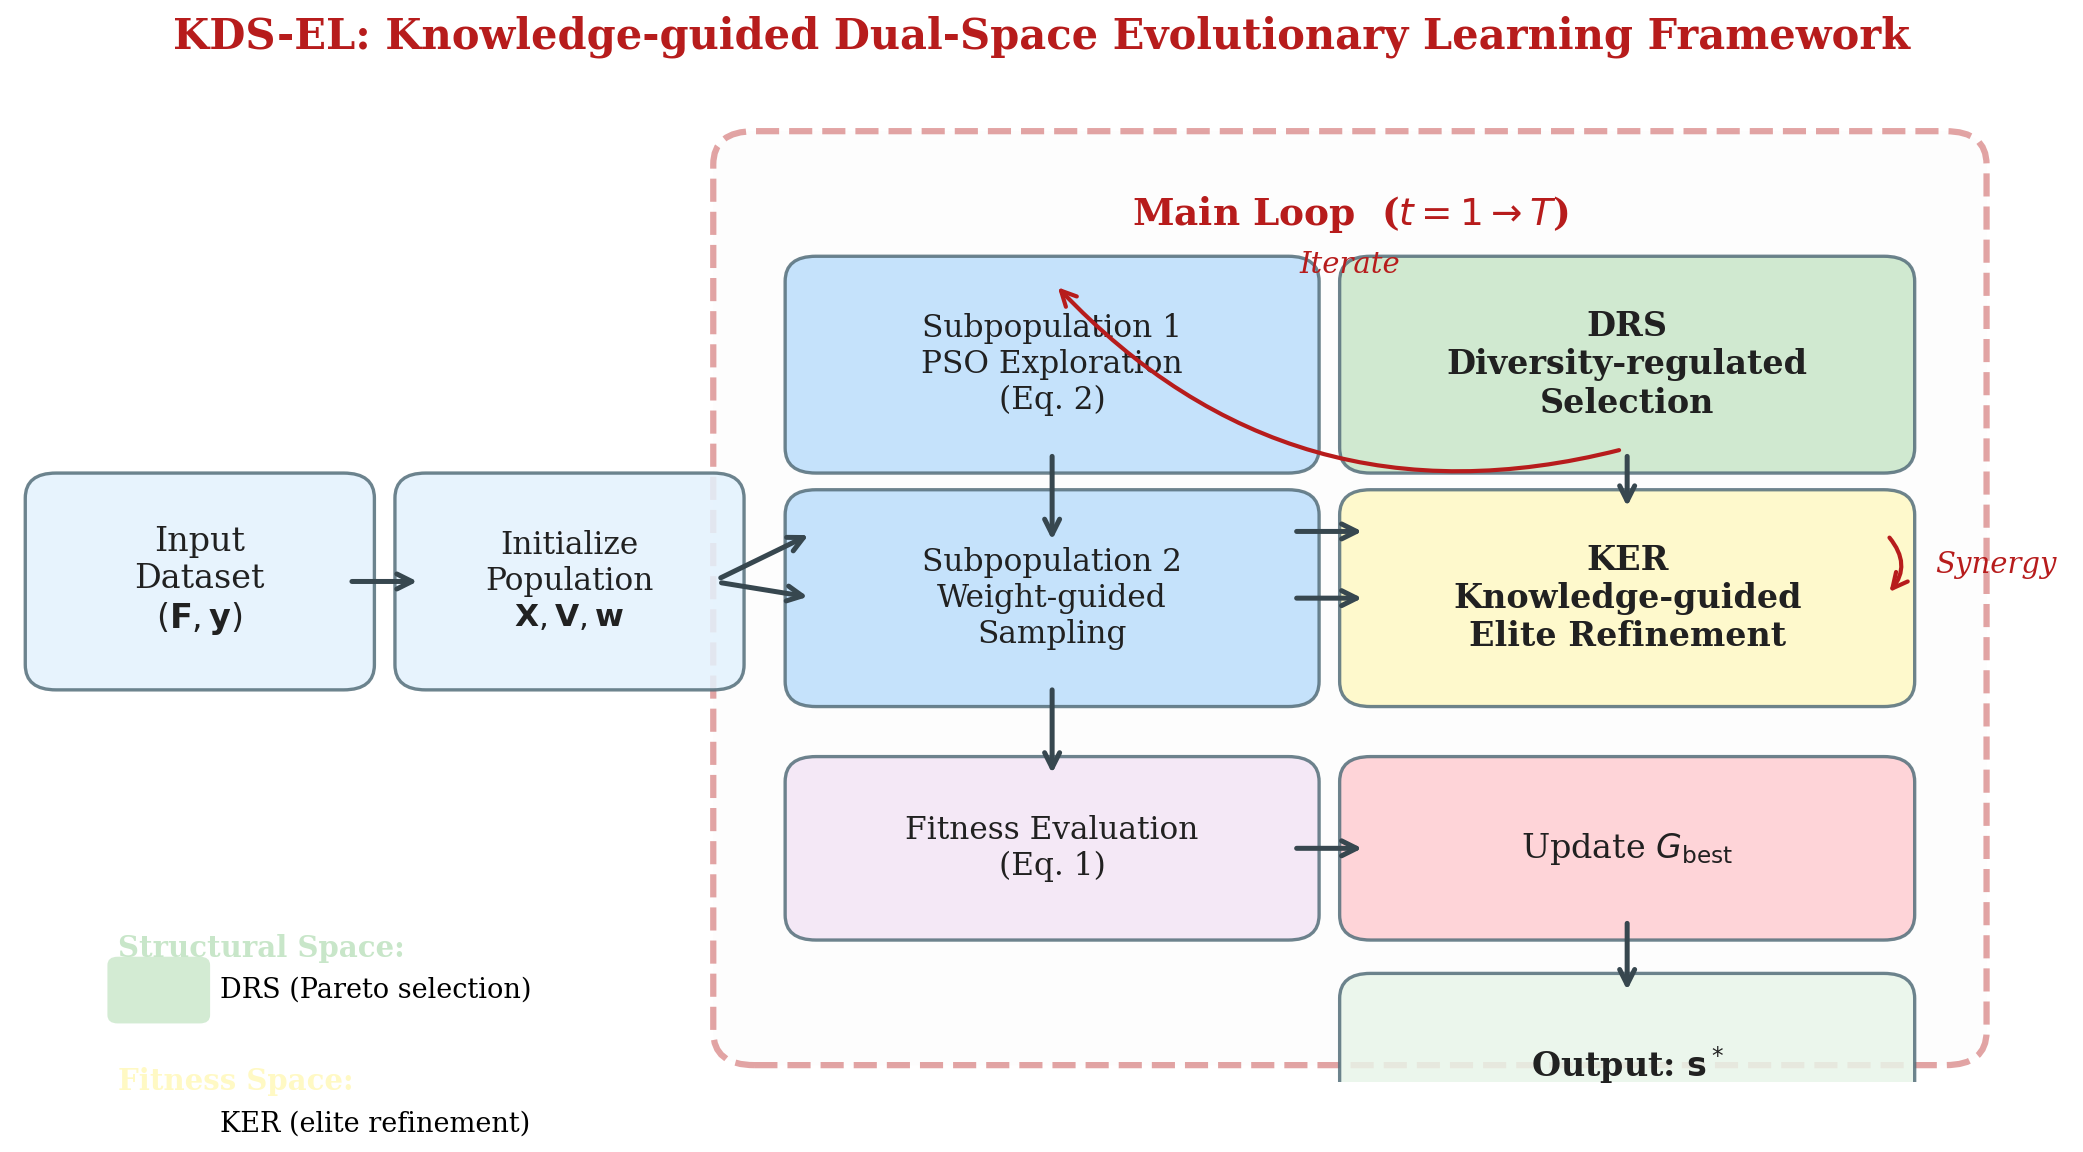
\includegraphics[width=0.85\textwidth]{../figures_new/fig1_framework.png}
	\caption{Overall architecture of the KDS-EL framework.
	The dual-space design operates in two complementary spaces:
	DRS (green, structural space) maintains population diversity via
	bi-objective Pareto selection, while KER (yellow, fitness space)
	accumulates improvement evidence to guide elite refinement.
	The two mechanisms are synergistically coupled across iterations.}
	\label{fig:framework}
	\end{figure*}

	\subsection{Problem Formulation}
	\label{sec:method:formulation}

	\par{
	Let $\mathcal{D} = \{(\mathbf{x}_i, y_i)\}_{i=1}^{n}$ denote a
	classification dataset with $n$ samples, where
	$\mathbf{x}_i \in \mathbb{R}^{d}$ is the feature vector and
	$y_i \in \{1, 2, \ldots, C\}$ is the class label.
	The feature selection problem seeks a binary mask
	$\mathbf{s} \in \{0,1\}^{d}$ that identifies a compact and
	informative feature subset.
	The wrapper-based fitness function used in this work is:
	\begin{equation}
		f(\mathbf{s}) = \alpha \cdot \mathcal{E}(\mathbf{s})
		+ (1 - \alpha) \cdot \frac{|\mathbf{s}|_1}{d},
		\label{eq:fitness}
	\end{equation}
	where $\mathcal{E}(\mathbf{s})$ is the classification error rate
	estimated via $K$-fold cross-validation using a $k$-nearest
	neighbour (KNN) classifier, $|\mathbf{s}|_1$ is the number of
	selected features, and $\alpha \in [0,1]$ controls the trade-off
	between accuracy and compactness.
	In this work, we set $\alpha = 0.9$, $K = 5$, and $k_{\mathrm{nn}} = 3$.
	}

	\subsection{Dual-Population PSO Backbone}
	\label{sec:method:backbone}

	\par{
	KDS-EL inherits the dual-subpopulation PSO architecture from
	MEL~\citep{MEL_CITE}, which partitions the swarm of $N$ particles
	into two equal-sized subpopulations.
	\textit{Subpopulation~1} (exploration) follows the standard PSO
	update rule with cognitive, social, and group-social acceleration
	coefficients $c_1$, $c_2$, and $c_3$:
	\begin{equation}
		\mathbf{v}_i^{(t+1)} = w \mathbf{v}_i^{(t)}
		+ c_1 r_1 (\mathbf{p}_i - \mathbf{x}_i^{(t)})
		+ c_2 r_2 (\mathbf{g} - \mathbf{x}_i^{(t)})
		+ c_3 r_3 (\mathbf{s}_k - \mathbf{x}_i^{(t)}),
		\label{eq:pso_update}
	\end{equation}
	where $w$ is the inertia weight, $r_1, r_2, r_3 \sim U(0,1)$,
	$\mathbf{p}_i$ is the personal best ($P_{\mathrm{best}}$),
	$\mathbf{g}$ is the global best ($G_{\mathrm{best}}$), and
	$\mathbf{s}_k$ is the best solution of the \emph{other} subpopulation.
	\textit{Subpopulation~2} (exploitation) samples new solutions from
	the feature-importance weight vector maintained by KER
	(Section~\ref{sec:method:ker}), with features selected
	probabilistically according to their accumulated importance.
	DRS and KER are the two novel components proposed in this work,
	and are detailed in the following subsections.
	}

	\subsection{Diversity-Regulated Selection (DRS)}
	\label{sec:method:drs}

	\par{
	The DRS operator addresses the structural collapse problem by
	elevating Normalised Hamming Distance (NHD) to a first-class Pareto
	selection objective.
	At each iteration $t$, DRS constructs a candidate pool by combining
	the current personal best solutions and newly generated solutions:
	\begin{equation}
		\mathcal{P} = \{P_{\mathrm{best}}^{(1)}, \ldots, P_{\mathrm{best}}^{(N)}\}
		\cup \{\mathbf{x}_1^{(t)}, \ldots, \mathbf{x}_N^{(t)}\},
		\label{eq:pool}
	\end{equation}
	yielding $|\mathcal{P}| = 2N$ candidates.
	Each candidate $\mathbf{s} \in \mathcal{P}$ is evaluated on two
	objectives:
	\begin{enumerate}
		\item \textbf{Objective 1} (minimise): fitness $f(\mathbf{s})$
		as defined in Eq.~\eqref{eq:fitness}.
		\item \textbf{Objective 2} (maximise): structural diversity
		quantified by the average NHD to all other solutions in the pool:
		\begin{equation}
			\mathrm{NHD}(\mathbf{s}) = \frac{1}{|\mathcal{P}|-1}
			\sum_{\mathbf{s}' \in \mathcal{P} \setminus \{\mathbf{s}\}}
			\frac{|\mathbf{s} \oplus \mathbf{s}'|_1}
			{\max(|\mathbf{s}|_1 + |\mathbf{s}'|_1 - 2|\mathbf{s} \cap \mathbf{s}'|_1, 1)},
			\label{eq:nhd}
		\end{equation}
		where $\oplus$ denotes the XOR operation and
		$|\mathbf{s} \cap \mathbf{s}'|_1$ counts the common selected features.
	\end{enumerate}

	\par{
	NSGA-II non-dominated sorting~\citep{deb2002fast} is applied to
	$\mathcal{P}$ to obtain Pareto fronts $\mathcal{F}_1, \mathcal{F}_2,
	\ldots$.
	Within each front, the crowding distance $\mathrm{CD}(\mathbf{s})$
	is computed in the standard manner.
	The final selection score combines the normalised crowding distance
	and the normalised NHD with an adaptive weight:
	\begin{equation}
		S(\mathbf{s}) = \alpha_{\mathrm{cd}}(t) \cdot
		\widetilde{\mathrm{CD}}(\mathbf{s})
		+ (1 - \alpha_{\mathrm{cd}}(t)) \cdot
		\widetilde{\mathrm{NHD}}(\mathbf{s}),
		\label{eq:selection_score}
	\end{equation}
	where $\widetilde{\cdot}$ denotes min-max normalisation across the
	front, and the adaptive schedule is:
	\begin{equation}
		\alpha_{\mathrm{cd}}(t) = \left(\frac{t}{T}\right)^2.
		\label{eq:alpha_cd}
	\end{equation}
	Early in the search ($t \ll T$), $\alpha_{\mathrm{cd}} \approx 0$
	and diversity dominates the selection; as $t \to T$,
	$\alpha_{\mathrm{cd}} \to 1$ and fitness precision takes priority.
	The top $N$ candidates by $S(\mathbf{s})$ are retained for the next
	iteration.
	}

	\par{
	\begin{proposition}[Diversity Lower Bound]
	\label{prop:drs}
	For any iteration $t < T$, the DRS operator guarantees that the
	selected population $\mathcal{S}^{(t)}$ satisfies:
	\begin{equation}
		\min_{\mathbf{s} \in \mathcal{S}^{(t)}} \mathrm{NHD}(\mathbf{s}) > 0.
	\end{equation}
	\end{proposition}
	\textit{Proof sketch.}
	For $t < T$, we have $\alpha_{\mathrm{cd}}(t) < 1$, so the NHD
	term contributes positively to the selection score
	$S(\mathbf{s})$ for every candidate with $\mathrm{NHD} > 0$.
	Since the candidate pool $\mathcal{P}$ contains $2N$ distinct
	binary vectors drawn from the evolving swarm, at least some
	candidates have strictly positive NHD.
	Any candidate with $\mathrm{NHD} = 0$ (a duplicate) receives a
	selection score of at most $\alpha_{\mathrm{cd}}(t) < 1$, while
	a non-duplicate with positive NHD can achieve a higher score.
	Therefore, duplicates are never strictly preferred over all
	non-duplicates, and the selected population maintains positive
	diversity. $\hfill\square$
	}

	Figure~\ref{fig:drs} illustrates the DRS mechanism, including the
	bi-objective Pareto selection process and the adaptive schedule
	$\alpha_{\mathrm{cd}}(t)$.

	\begin{figure*}[t]
	\centering
	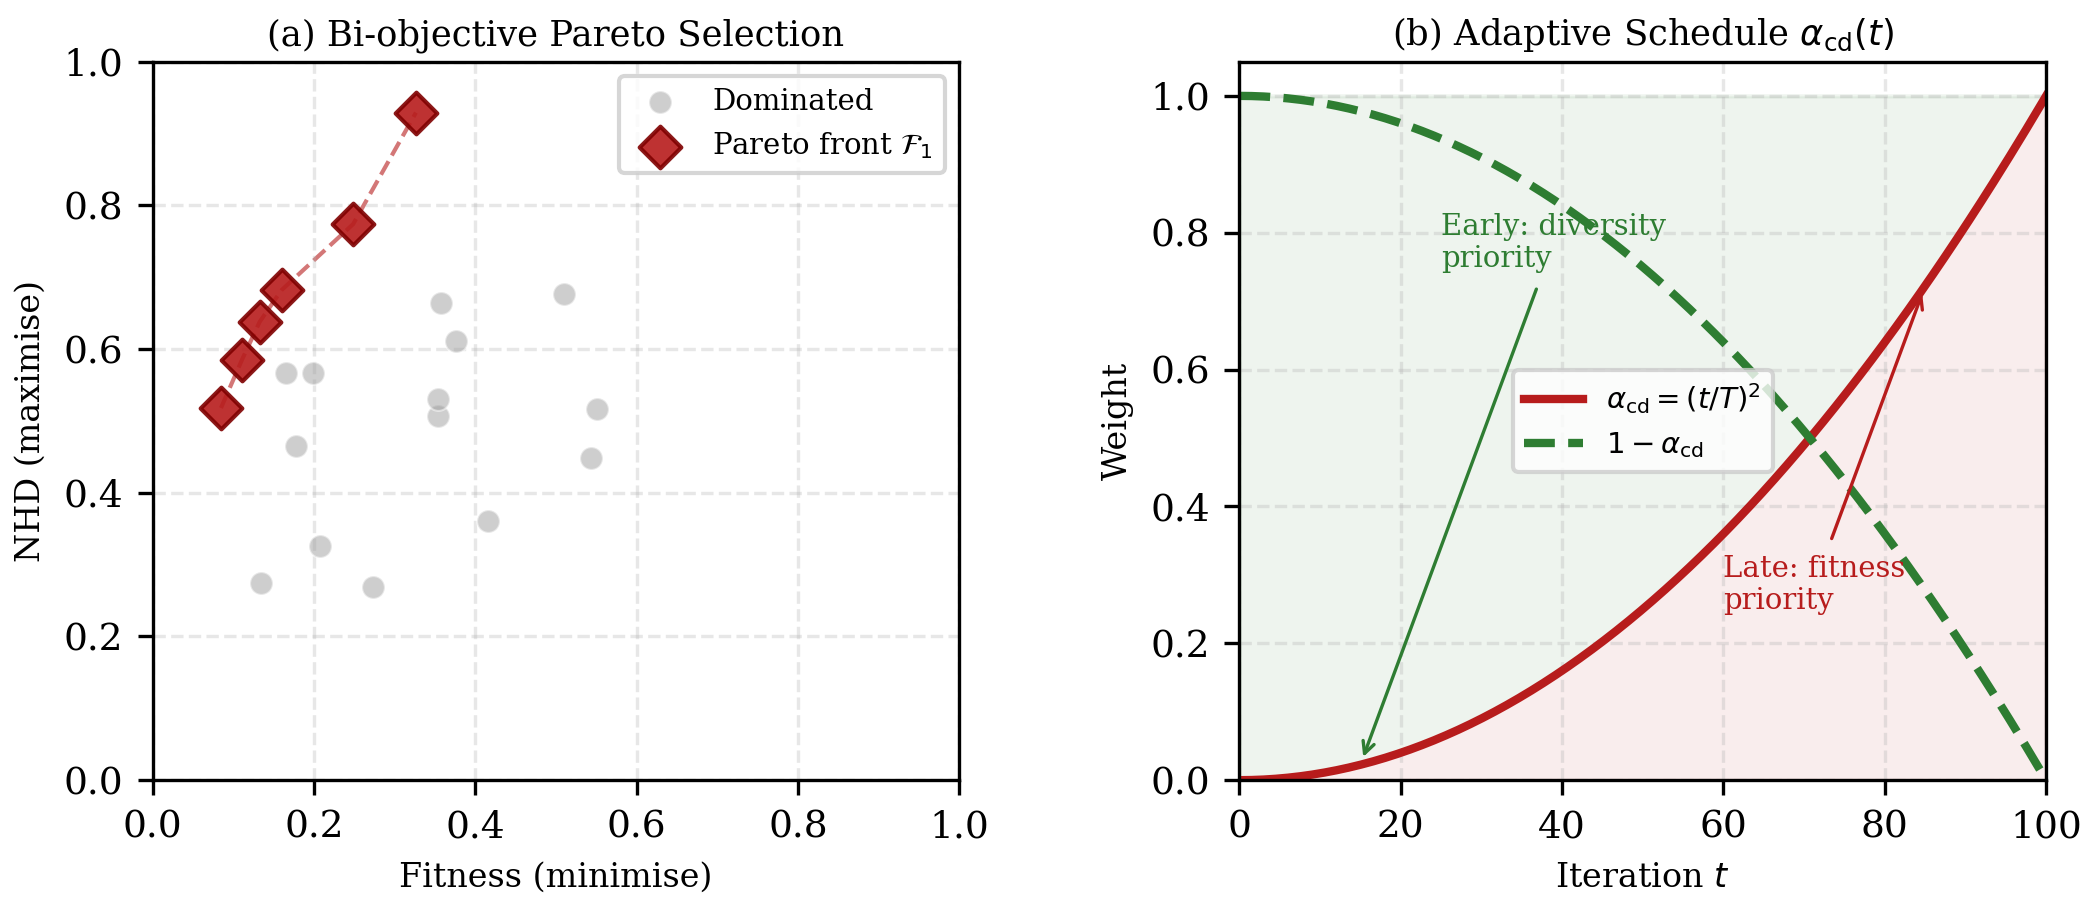
\includegraphics[width=0.85\textwidth]{../figures_new/fig2_drs_mechanism.png}
	\caption{Illustration of the DRS mechanism.
	(a)~Bi-objective Pareto selection: solutions are sorted by fitness
	and NHD, with the Pareto front $\mathcal{F}_1$ receiving priority.
	(b)~Adaptive schedule $\alpha_{\mathrm{cd}}(t) = (t/T)^2$:
	early iterations prioritise diversity (green region), while later
	iterations prioritise fitness precision (red region).}
	\label{fig:drs}
	\end{figure*}

	\subsection{Knowledge-Guided Elite Refinement (KER)}
	\label{sec:method:ker}

	\par{
	The KER mechanism addresses the knowledge waste problem by
	accumulating improvement-event evidence from the evolutionary
	trajectory into a feature-importance weight vector
	$\mathbf{w} \in \mathbb{R}^d$.
	At each iteration, after evaluating all particles, KER performs
	the following steps for each particle $i$ that improved:
	}

	\par{
	\textbf{Step~1: Weight Update.}
	Let $\Delta = f(P_{\mathrm{best}}^{(i)}) - f(\mathbf{x}_i^{(t)})$
	denote the fitness improvement.
	Let $\mathbf{s}_{\mathrm{new}}$ and $\mathbf{s}_{\mathrm{old}}$ denote
	the binary masks of the new solution and $P_{\mathrm{best}}$,
	respectively.
	The weight update is:
	\begin{equation}
		w_j \leftarrow \begin{cases}
			w_j + \Delta & \text{if feature } j \text{ was added (0$\to$1)}, \\
			w_j - \Delta & \text{if feature } j \text{ was removed (1$\to$0)}, \\
			w_j           & \text{otherwise}.
		\end{cases}
		\label{eq:weight_update}
	\end{equation}
	\textbf{Crucially}, this weight update is performed \emph{before}
	$P_{\mathrm{best}}$ is updated, ensuring that the improvement
	signal is captured while the comparison is still valid.
	}

	\par{
	\textbf{Step~2: Elite Perturbation.}
	For the top $k_e = 3$ particles by fitness improvement, KER
	generates a mutant solution via guided bit-flip perturbation.
	With probability $p_r = 0.10$, each bit is flipped uniformly at
	random (guaranteeing ergodicity); otherwise, the flip probability
	is guided by the weight vector:
	\begin{equation}
		p_j^{\mathrm{flip}} \propto \begin{cases}
			|w_j| & \text{if } w_j > 0 \text{ and } s_j = 0
			\text{ (add valuable feature)}, \\
			|w_j| & \text{if } w_j < 0 \text{ and } s_j = 1
			\text{ (remove harmful feature)}, \\
			\epsilon & \text{otherwise},
		\end{cases}
		\label{eq:flip_prob}
	\end{equation}
	where $\epsilon$ is a small positive constant.
	The top-$k$ features by flip probability are flipped to produce
	the mutant.
	If the mutant improves upon the corresponding $P_{\mathrm{best}}$,
	it replaces it.
	}

	\par{
	\begin{proposition}[Ergodicity]
	\label{prop:ker}
	With probability $p_r > 0$ at each bit position and each iteration,
	KER can reach any binary mask $\mathbf{s} \in \{0,1\}^d$ in
	finitely many steps, ensuring ergodicity of the induced Markov chain.
	\end{proposition}
	\textit{Proof sketch.}
	The random-flip branch with probability $p_r > 0$ at each bit
	position implies that the transition probability from any state
	to any other state is strictly positive.
	By the ergodic theorem for finite Markov chains, the chain is
	irreducible and aperiodic, hence ergodic. $\hfill\square$
	}

	Figure~\ref{fig:ker} illustrates the KER mechanism, including the
	improvement-feedback weight update process and the elite perturbation
	with ergodicity guarantee.

	\begin{figure*}[t]
	\centering
	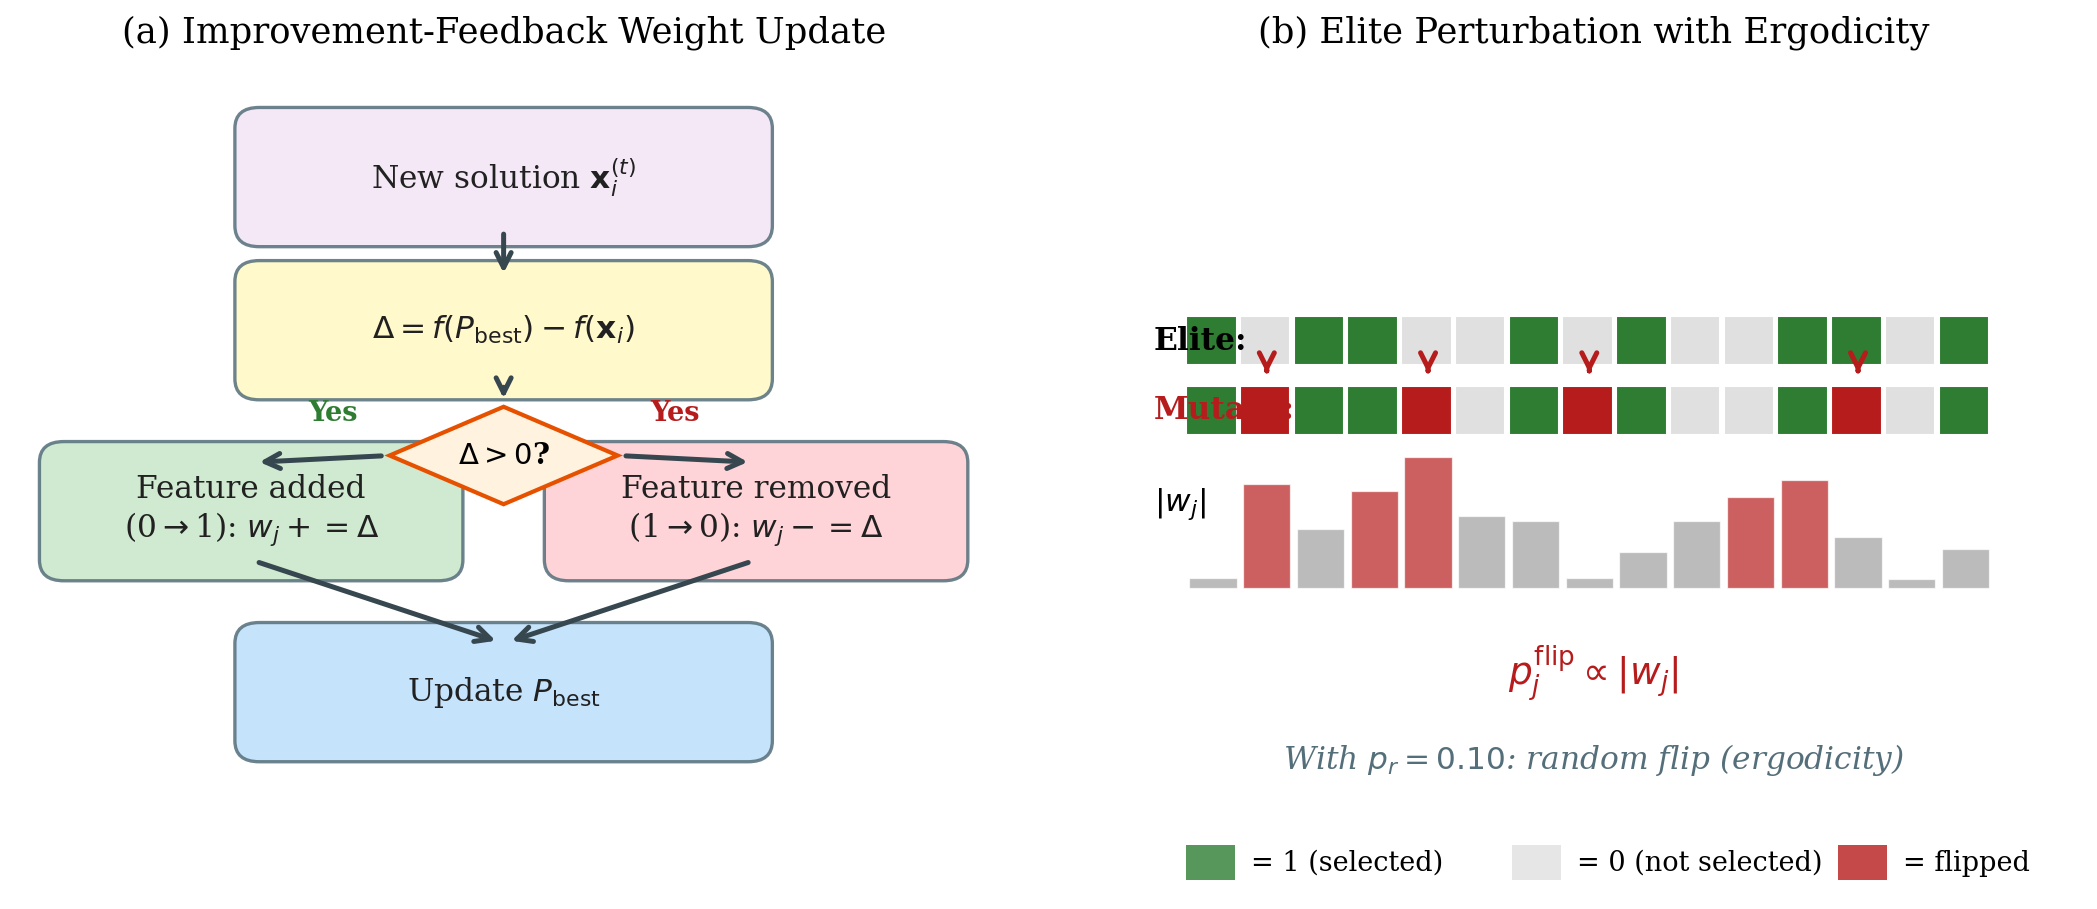
\includegraphics[width=0.85\textwidth]{../figures_new/fig3_ker_mechanism.png}
	\caption{Illustration of the KER mechanism.
	(a)~Improvement-feedback weight update: when a new solution improves
	upon $P_{\mathrm{best}}$, the weight vector $\mathbf{w}$ is updated
	before $P_{\mathrm{best}}$ is replaced.
	(b)~Elite perturbation: features with high $|w_j|$ have higher flip
	probability, while random flips with probability $p_r = 0.10$
	guarantee ergodicity.}
	\label{fig:ker}
	\end{figure*}

	\subsection{Complete KDS-EL Algorithm}
	\label{sec:method:complete}

	\par{
	Algorithm~\ref{alg:kdsel} presents the complete KDS-EL procedure.
	The algorithm begins by initialising the population, velocity,
	and weight vectors.
	At each iteration, Subpopulation~1 updates via standard PSO
	(Eq.~\eqref{eq:pso_update}) while Subpopulation~2 samples from
	the weight vector.
	After fitness evaluation, DRS performs bi-objective selection,
	and KER accumulates improvement evidence and generates elite
	perturbations.
	The algorithm terminates after $T$ iterations and returns the
	global best solution $G_{\mathrm{best}}$.
	}

	\begin{algorithm}[t]
	\caption{KDS-EL: Knowledge-guided Dual-Space Evolutionary Learning}
	\label{alg:kdsel}
	\hspace*{0.02in} {\bf Input:}
	Feature matrix $\mathbf{F}$, label vector $\mathbf{y}$,
	swarm size $N$, max iterations $T$, threshold $\theta$.\\
	\hspace*{0.02in} {\bf Output:}
	Best feature subset $\mathbf{s}^*$.
	\begin{algorithmic}[1]
		\State Initialise $\mathbf{X}, \mathbf{V} \in \mathbb{R}^{N \times d}$,
		$\mathbf{w} \leftarrow \mathbf{0}$,
		$G_{\mathrm{best}} \leftarrow \infty$
		\State Evaluate fitness $f(\mathbf{x}_i)$ for all $i$; set
		$P_{\mathrm{best}}^{(i)} \leftarrow \mathbf{x}_i$
		\For{$t = 1 \to T$}
			\For{each particle $i \in \{1,\ldots,N\}$}
				\If{$i \leq N/2$} \Comment{Subpopulation 1: PSO}
					\State Update $\mathbf{v}_i$ via Eq.~\eqref{eq:pso_update}
					\State Update $\mathbf{x}_i \leftarrow \mathbf{x}_i + \mathbf{v}_i$
				\Else \Comment{Subpopulation 2: Weight-guided sampling}
					\State Sample $\mathbf{x}_i$ from $\mathbf{w}$ probabilistically
				\EndIf
				\State Evaluate $f(\mathbf{x}_i)$
			\EndFor
			\State \textbf{DRS:} Construct pool $\mathcal{P}$ (Eq.~\eqref{eq:pool})
			\State \textbf{DRS:} Pareto sort + selection score (Eq.~\eqref{eq:selection_score})
			\State \textbf{DRS:} Select top $N$ candidates
			\For{each improved particle $i$}
				\State \textbf{KER:} Update $\mathbf{w}$ via Eq.~\eqref{eq:weight_update}
				\State \textbf{KER:} Update $P_{\mathrm{best}}^{(i)} \leftarrow \mathbf{x}_i$
			\EndFor
			\State \textbf{KER:} Elite perturbation for top-$k_e$ particles (Eq.~\eqref{eq:flip_prob})
			\State Update $G_{\mathrm{best}}$ if any $P_{\mathrm{best}}^{(i)}$ improved
		\EndFor
		\State $\mathbf{s}^* \leftarrow G_{\mathrm{best}} > \theta$
		\State \Return $\mathbf{s}^*$
	\end{algorithmic}
	\end{algorithm}


	\subsection{Time Complexity Analysis}
	\label{sec:method:complexity}

	\par{
	The per-iteration time complexity of KDS-EL is dominated by two
	components:
	(i)~fitness evaluation, which requires $O((2N + k_e) \cdot C_f)$
	where $C_f$ is the cost of a single KNN cross-validation; and
	(ii)~DRS's pairwise NHD computation, which requires $O(N^2 \cdot d)$.
	The total complexity over $T$ iterations is:
	\begin{equation}
		O\bigl(T \cdot (2N + k_e) \cdot C_f + T \cdot N^2 \cdot d\bigr).
		\label{eq:complexity}
	\end{equation}
	Since $N = 20$ and $k_e = 3$ are small constants, and $C_f = O(K
	\cdot n \cdot d_{\mathrm{sel}} / K)$, the dominant term in practice
	is the fitness evaluation.
	Compared to BPSO and SaWDE (which perform $N \times T = 2000$
	evaluations), KDS-EL performs $(2N + k_e) \times T = 4300$
	evaluations---a 2.15$\times$ increase that is the deliberate cost
	of DRS's pool construction and KER's elite perturbation.
	This additional cost is offset by KDS-EL's superior accuracy and
	dramatic feature reduction, as demonstrated in
	Section~\ref{sec:experiments}.
	}

	% ════════════════════════════════════════════════════════════════════════
	%  4. EXPERIMENTS
	% ════════════════════════════════════════════════════════════════════════

	\section{Experimental Results and Discussion}
	\label{sec:experiments}

	\subsection{Experimental Setup}
	\label{sec:experiments:setup}

	\subsubsection{Datasets}
	\label{sec:experiments:datasets}

	\par{
	Nine high-dimensional bioinformatics datasets are used in this
	study, spanning a wide range of sample sizes ($n \in [60, 2500]$),
	feature dimensions ($d \in [2000, 26877]$), and class counts
	($C \in \{2, 9\}$).
	Table~\ref{tab:datasets} summarises the characteristics of each
	dataset.
	These datasets cover diverse bioinformatics applications including
	cancer classification (Colon, DLBCL, Leukaemia, ALL4), tissue
	identification (Adenoma, ALL-AML, Lymphoma), and disease diagnosis
	(CNS, Stroke), providing a comprehensive evaluation benchmark.
	}

	\begin{table}[t]
	\centering
	\caption{Summary of the nine bioinformatics datasets used in experiments.}
	\label{tab:datasets}
	\setlength{\tabcolsep}{4pt}
	\begin{tabular}{lrrrl}
	\toprule
	\textbf{Dataset} & \textbf{$n$} & \textbf{$d$} & \textbf{$C$} & \textbf{Domain} \\
	\midrule
	Adenoma     & 36   & 3,408  & 2 & Tissue identification \\
	ALL-AML     & 72   & 7,129  & 2 & Leukaemia subtype \\
	ALL4        & 102  & 9,999  & 2 & Leukaemia subtype \\
	CNS         & 60   & 7,129  & 2 & Brain tumour \\
	Colon       & 62   & 2,000  & 2 & Colon cancer \\
	DLBCL       & 77   & 5,469  & 2 & Lymphoma subtype \\
	Leukaemia   & 72   & 7,129  & 2 & Leukaemia \\
	Lymphoma    & 96   & 4,026  & 9 & Lymphoma \\
	Stroke      & 2,500 & 26,877 & 2 & Disease diagnosis \\
	\bottomrule
	\end{tabular}
	\end{table}


	\subsubsection{Comparison Algorithms}
	\label{sec:experiments:algorithms}

	\par{
	Eight state-of-the-art methods are selected for comparison,
	covering classical baselines, recent PSO variants, and ablation
	variants of KDS-EL:
	\begin{enumerate}
		\item \textbf{BPSO}~\citep{chuang2011binary}: Standard binary PSO
		with sigmoid transfer function.
		\item \textbf{SaWDE}~\citep{zhan2020sa}: Self-adaptive
		weighted differential evolution.
		\item \textbf{FWPSO}~\citep{huang2020enhanced}: Feature-weight-based
		PSO with importance-biased initialisation.
		\item \textbf{MEL}~\citep{MEL_CITE}: Multi-task evolutionary
		learning with dual subpopulations (the base framework).
		\item \textbf{KDS-EL/DRS}: Ablation variant with only the DRS
		operator (no KER).
		\item \textbf{KDS-EL/KER}: Ablation variant with only the KER
		mechanism (no DRS).
		\item \textbf{PSO-CSM}~(2025)~\citep{PSOCSM_CITE}: PSO with
		comprehensive scoring metric.
		\item \textbf{IGPSO}~(2024)~\citep{IGPSO_CITE}: PSO with
		MLP-based feature importance pre-training.
	\end{enumerate}
	The full KDS-EL (with both DRS and KER) is the proposed method.
	}


	\subsubsection{Parameter Settings}
	\label{sec:experiments:params}

	\par{
	Table~\ref{tab:params} lists the parameter settings for all
	algorithms.
	For fairness, common parameters (swarm size $N$, maximum iterations
	$T$, KNN settings) are identical across all methods.
	KDS-EL-specific parameters ($p_r$, $k_e$, $\alpha_{\mathrm{cd}}$
	schedule) are inherited from the MEL baseline or set to standard
	defaults.
	}

	\begin{table}[t]
	\centering
	\caption{Parameter settings for all algorithms.}
	\label{tab:params}
	\setlength{\tabcolsep}{4pt}
	\begin{tabular}{lll}
	\toprule
	\textbf{Parameter} & \textbf{Value} & \textbf{Description} \\
	\midrule
	$N$          & 20    & Swarm size \\
	$T$          & 100   & Maximum iterations \\
	$K$          & 5     & CV folds \\
	$k_{\mathrm{nn}}$ & 3  & KNN neighbours \\
	$\theta$     & 0.6   & Binary threshold \\
	$\alpha$     & 0.9   & Fitness weight (accuracy) \\
	$w$          & 0.9   & Inertia weight \\
	$c_1, c_2, c_3$ & 2  & Acceleration coefficients \\
	$p_r$        & 0.10  & Random flip probability (KER) \\
	$k_e$        & 3     & Elite perturbation count (KER) \\
	$\alpha_{\mathrm{cd}}(t)$ & $(t/T)^2$ & Adaptive schedule (DRS) \\
	Runs         & 10    & Independent runs \\
	Seeds        & $42 + \text{run} \times 37$ & Reproducibility \\
	\bottomrule
	\end{tabular}
	\end{table}


	\subsubsection{Evaluation Protocol}
	\label{sec:experiments:protocol}

	\par{
	Each algorithm is evaluated using stratified 5-fold cross-validation
	(StratifiedKFold with shuffle=True, random\_state=42) repeated over
	10 independent runs with seeds $42 + \text{run} \times 37$ for
	reproducibility.
	Performance is measured by classification accuracy (mean $\pm$
	standard deviation), number of selected features, and runtime.
	Statistical significance is assessed using the Friedman test for
	global comparison and the Wilcoxon signed-rank test for pairwise
	comparison, with a significance level of $\alpha = 0.05$.
	}

	\subsection{Classification Accuracy Comparison}
	\label{sec:experiments:accuracy}

	\par{
	Table~\ref{tab:accuracy} and Figure~\ref{fig:accuracy} present the
	mean classification accuracy and standard deviation for all nine
	methods across the nine datasets.
	KDS-EL achieves the highest mean accuracy on 7 of 9 datasets,
	with an overall average of 93.28\% and an average Friedman rank of
	1.222.
	The Friedman test yields $\chi^2 = 47.38$ with
	$p = 1.30 \times 10^{-7}$, confirming statistically significant
	differences among the methods.
	}

	% ─────────────────────────────────────────────────────────────
% Table 4: Classification Accuracy (mean ± std)
% Bold = best, underline = second-best per dataset
% ─────────────────────────────────────────────────────────────
\begin{table*}[t]
\centering
\caption{Comparison of mean classification accuracy (\%) and standard deviation.
Bold values indicate the best result; underlined values indicate the second-best.}
\label{tab:accuracy}
\setlength{\tabcolsep}{3.5pt}
\begin{tabular}{lccccccccc}
\toprule
\textbf{Dataset} & \textbf{BPSO} & \textbf{SaWDE} & \textbf{FWPSO} & \textbf{MEL} & \textbf{KDS-EL/DRS} & \textbf{KDS-EL/KER} & \textbf{KDS-EL} & \textbf{PSO-CSM} & \textbf{IGPSO} \\
\midrule
Adenoma & 92.86$\pm$0.02 & 94.88$\pm$0.79 & \underline{98.23$\pm$1.37} & 97.34$\pm$2.52 & 97.70$\pm$2.43 & 95.78$\pm$2.03 & \textbf{98.37$\pm$1.42} & 96.39$\pm$0.73 & 95.52$\pm$0.74 \\
ALL-AML & 94.16$\pm$0.02 & 96.11$\pm$0.47 & \underline{98.49$\pm$0.68} & 95.61$\pm$0.63 & 96.14$\pm$1.01 & 97.29$\pm$1.66 & \textbf{99.25$\pm$0.78} & 97.36$\pm$0.01 & 96.71$\pm$0.02 \\
ALL4 & 75.23$\pm$0.75 & 80.52$\pm$1.32 & 85.07$\pm$4.23 & 81.75$\pm$2.41 & 82.74$\pm$2.77 & \underline{86.65$\pm$2.17} & \textbf{88.22$\pm$2.61} & 83.41$\pm$0.86 & 78.65$\pm$1.11 \\
CNS & 75.89$\pm$0.77 & 80.07$\pm$1.01 & \textbf{82.20$\pm$2.43} & 78.23$\pm$1.50 & 79.80$\pm$2.65 & 81.07$\pm$2.68 & \underline{81.31$\pm$2.31} & 73.67$\pm$1.20 & 71.95$\pm$1.28 \\
Colon & 85.05$\pm$0.50 & 88.20$\pm$0.91 & 91.00$\pm$1.99 & 87.37$\pm$2.46 & 85.63$\pm$2.04 & \underline{91.21$\pm$2.55} & \textbf{93.05$\pm$2.10} & 89.20$\pm$0.63 & 86.34$\pm$1.16 \\
DLBCL & 94.18$\pm$0.04 & 96.36$\pm$0.55 & \underline{98.50$\pm$0.90} & 95.28$\pm$0.62 & 95.23$\pm$1.37 & 98.11$\pm$1.43 & \textbf{99.13$\pm$0.77} & 98.05$\pm$0.52 & 96.54$\pm$0.62 \\
Leukaemia & 94.93$\pm$0.06 & 93.74$\pm$0.04 & 93.92$\pm$0.02 & 95.65$\pm$0.66 & \textbf{97.35$\pm$0.87} & 96.29$\pm$1.20 & \underline{96.79$\pm$1.60} & 94.91$\pm$0.06 & 93.97$\pm$0.02 \\
Lymphoma & 86.21$\pm$0.92 & 88.59$\pm$0.73 & \underline{94.42$\pm$2.16} & 88.41$\pm$3.21 & 89.90$\pm$3.02 & 92.83$\pm$2.71 & \textbf{95.54$\pm$1.93} & 92.23$\pm$1.15 & 88.61$\pm$1.00 \\
Stroke & 77.08$\pm$1.41 & 81.34$\pm$1.36 & \underline{85.31$\pm$3.77} & 81.95$\pm$4.60 & 83.31$\pm$3.95 & 84.61$\pm$3.21 & \textbf{87.87$\pm$1.80} & 76.04$\pm$0.58 & 75.13$\pm$1.02 \\
\midrule
\textbf{Average} & 86.18 & 88.87 & \underline{91.91} & 89.06 & 89.76 & 91.54 & \textbf{93.28} & 89.03 & 87.05 \\
\textbf{Avg. Rank} & 8.111 & 6.556 & \underline{2.778} & 6.000 & 5.000 & 3.222 & \textbf{1.222} & 5.111 & 7.000 \\
\midrule
\multicolumn{10}{l}{Friedman test: $\chi^2=47.38$, $p=1.30e-07$} \\
\bottomrule
\end{tabular}
\end{table*}

% ─────────────────────────────────────────────────────────────
% Table 5: Number of Selected Features (mean)
% ─────────────────────────────────────────────────────────────
\begin{table*}[t]
\centering
\caption{Comparison of the mean number of selected features.
Bold values indicate the fewest features; underlined values indicate the second-fewest.}
\label{tab:features}
\setlength{\tabcolsep}{3.5pt}
\begin{tabular}{lccccccccc}
\toprule
\textbf{Dataset} & \textbf{BPSO} & \textbf{SaWDE} & \textbf{FWPSO} & \textbf{MEL} & \textbf{KDS-EL/DRS} & \textbf{KDS-EL/KER} & \textbf{KDS-EL} & \textbf{PSO-CSM} & \textbf{IGPSO} \\
\midrule
Adenoma & 3,408 & 2,094 & \underline{358} & 1,028 & 756 & 1,609 & \textbf{260} & 1,129 & 1,618 \\
ALL-AML & 3,248 & 2,041 & \underline{526} & 2,124 & 1,836 & 1,290 & \textbf{258} & 931 & 1,427 \\
ALL4 & 6,217 & 4,466 & 1,280 & \underline{685} & 778 & 871 & \textbf{491} & 1,436 & 2,677 \\
CNS & 3,540 & 2,666 & 1,092 & \underline{592} & \textbf{431} & 1,559 & 1,094 & 2,664 & 2,589 \\
Colon & 927 & 601 & 263 & 364 & 490 & \underline{218} & \textbf{126} & 284 & 456 \\
DLBCL & 3,349 & 2,272 & \underline{737} & 2,038 & 1,659 & 855 & \textbf{371} & 1,084 & 1,700 \\
Leukaemia & 2,700 & 3,548 & 3,414 & 2,095 & \textbf{704} & 1,728 & \underline{1,463} & 2,699 & 3,380 \\
Lymphoma & 1,848 & 1,212 & 396 & 802 & 604 & \underline{391} & \textbf{186} & 540 & 883 \\
Stroke & 26,877 & 18,383 & 6,485 & 6,448 & 7,625 & \underline{4,168} & \textbf{1,105} & 17,490 & 21,557 \\
\midrule
\textbf{Average} & 5,790 & 4,143 & 1,617 & 1,797 & 1,654 & \underline{1,410} & \textbf{595} & 3,140 & 4,032 \\
\bottomrule
\end{tabular}
\end{table*}

% ─────────────────────────────────────────────────────────────
% Table 6: Wilcoxon Signed-Rank Test p-values
% Bold = p > 0.05 (not significant); underline = 0.01 < p ≤ 0.05
% ─────────────────────────────────────────────────────────────
\begin{table*}[t]
\centering
\caption{$p$-values of the Wilcoxon signed-rank test between KDS-EL and each competitor.
Bold values denote $p>0.05$ (not significant); underlined values denote $0.01<p\leq0.05$.}
\label{tab:wilcoxon}
\setlength{\tabcolsep}{4pt}
\begin{tabular}{lcccccccc}
\toprule
\textbf{Dataset} & \textbf{BPSO} & \textbf{SaWDE} & \textbf{FWPSO} & \textbf{MEL} & \textbf{KDS-EL/DRS} & \textbf{KDS-EL/KER} & \textbf{PSO-CSM} & \textbf{IGPSO} \\
\midrule
Adenoma & 0.0020 & 0.0039 & \textbf{0.6250} & \textbf{0.3223} & \textbf{0.7695} & 0.0039 & \underline{0.0195} & 0.0039 \\
ALL-AML & 0.0020 & 0.0020 & \textbf{0.0840} & 0.0020 & 0.0020 & \underline{0.0273} & 0.0020 & 0.0020 \\
ALL4 & 0.0020 & 0.0020 & \textbf{0.1602} & 0.0039 & 0.0098 & \textbf{0.3223} & 0.0020 & 0.0020 \\
CNS & 0.0020 & \textbf{0.2324} & \textbf{0.4922} & \underline{0.0195} & \textbf{0.2324} & \textbf{0.8457} & 0.0020 & 0.0020 \\
Colon & 0.0020 & 0.0039 & \underline{0.0195} & 0.0098 & 0.0020 & \textbf{0.0840} & 0.0039 & 0.0020 \\
DLBCL & 0.0020 & 0.0020 & \textbf{0.0645} & 0.0020 & 0.0020 & \textbf{0.1055} & \underline{0.0195} & 0.0020 \\
Leukaemia & 0.0020 & 0.0020 & 0.0020 & \textbf{0.0742} & \textbf{0.2500} & \textbf{0.6953} & 0.0020 & 0.0020 \\
Lymphoma & 0.0020 & 0.0020 & \textbf{0.4316} & 0.0059 & 0.0039 & \textbf{0.0645} & 0.0020 & 0.0020 \\
Stroke & 0.0020 & 0.0020 & \underline{0.0273} & 0.0039 & 0.0098 & \underline{0.0195} & 0.0020 & 0.0020 \\
\bottomrule
\end{tabular}
\end{table*}

% ─────────────────────────────────────────────────────────────
% Table 7: Ablation Study
% ─────────────────────────────────────────────────────────────
\begin{table*}[t]
\centering
\caption{Ablation study results. For each dataset, accuracy (mean\,$\pm$\,std, \%) and
number of selected features (mean) are reported for four variants.
Bold = best accuracy; $\dagger$ = best feature count per dataset.}
\label{tab:ablation}
\setlength{\tabcolsep}{4pt}
\begin{tabular}{lcccccccc}
\toprule
\textbf{Dataset} & \multicolumn{2}{c}{\textbf{MEL}} & \multicolumn{2}{c}{\textbf{KDS-EL/DRS}} & \multicolumn{2}{c}{\textbf{KDS-EL/KER}} & \multicolumn{2}{c}{\textbf{KDS-EL}} \\
\cmidrule(lr){2-3}\cmidrule(lr){4-5}\cmidrule(lr){6-7}\cmidrule(lr){8-9}
 & Acc. & Feat. & Acc. & Feat. & Acc. & Feat. & Acc. & Feat. \\
\midrule
Adenoma & 97.34$\pm$2.52 & 1,028 & 97.70$\pm$2.43 & 756 & 95.78$\pm$2.03 & 1,609 & \textbf{98.37$\pm$1.42} & 260$^\dagger$ \\
ALL-AML & 95.61$\pm$0.63 & 2,124 & 96.14$\pm$1.01 & 1,836 & 97.29$\pm$1.66 & 1,290 & \textbf{99.25$\pm$0.78} & 258$^\dagger$ \\
ALL4 & 81.75$\pm$2.41 & 685 & 82.74$\pm$2.77 & 778 & 86.65$\pm$2.17 & 871 & \textbf{88.22$\pm$2.61} & 491$^\dagger$ \\
CNS & 78.23$\pm$1.50 & 592 & 79.80$\pm$2.65 & 431$^\dagger$ & 81.07$\pm$2.68 & 1,559 & \textbf{81.31$\pm$2.31} & 1,094 \\
Colon & 87.37$\pm$2.46 & 364 & 85.63$\pm$2.04 & 490 & 91.21$\pm$2.55 & 218 & \textbf{93.05$\pm$2.10} & 126$^\dagger$ \\
DLBCL & 95.28$\pm$0.62 & 2,038 & 95.23$\pm$1.37 & 1,659 & 98.11$\pm$1.43 & 855 & \textbf{99.13$\pm$0.77} & 371$^\dagger$ \\
Leukaemia & 95.65$\pm$0.66 & 2,095 & \textbf{97.35$\pm$0.87} & 704$^\dagger$ & 96.29$\pm$1.20 & 1,728 & 96.79$\pm$1.60 & 1,463 \\
Lymphoma & 88.41$\pm$3.21 & 802 & 89.90$\pm$3.02 & 604 & 92.83$\pm$2.71 & 391 & \textbf{95.54$\pm$1.93} & 186$^\dagger$ \\
Stroke & 81.95$\pm$4.60 & 6,448 & 83.31$\pm$3.95 & 7,625 & 84.61$\pm$3.21 & 4,168 & \textbf{87.87$\pm$1.80} & 1,105$^\dagger$ \\
\midrule
\multicolumn{9}{l}{\textit{Synergy} ($\Delta_\text{Full} - \Delta_\text{DRS} - \Delta_\text{KER}$):} \\
 & \multicolumn{8}{l}{\textit{Adenoma}: $+$2.217~~\textit{ALL-AML}: $+$1.430~~\textit{ALL4}: $+$0.575~~\textit{CNS}: $-$1.339~~\textit{Colon}: $+$3.566~~\textit{DLBCL}: $+$1.063~~\textit{Leukaemia}: $-$1.203~~\textit{Lymphoma}: $+$1.219~~\textit{Stroke}: $+$1.900} \\
\bottomrule
\end{tabular}
\end{table*}

	\begin{figure*}[t]
	\centering
	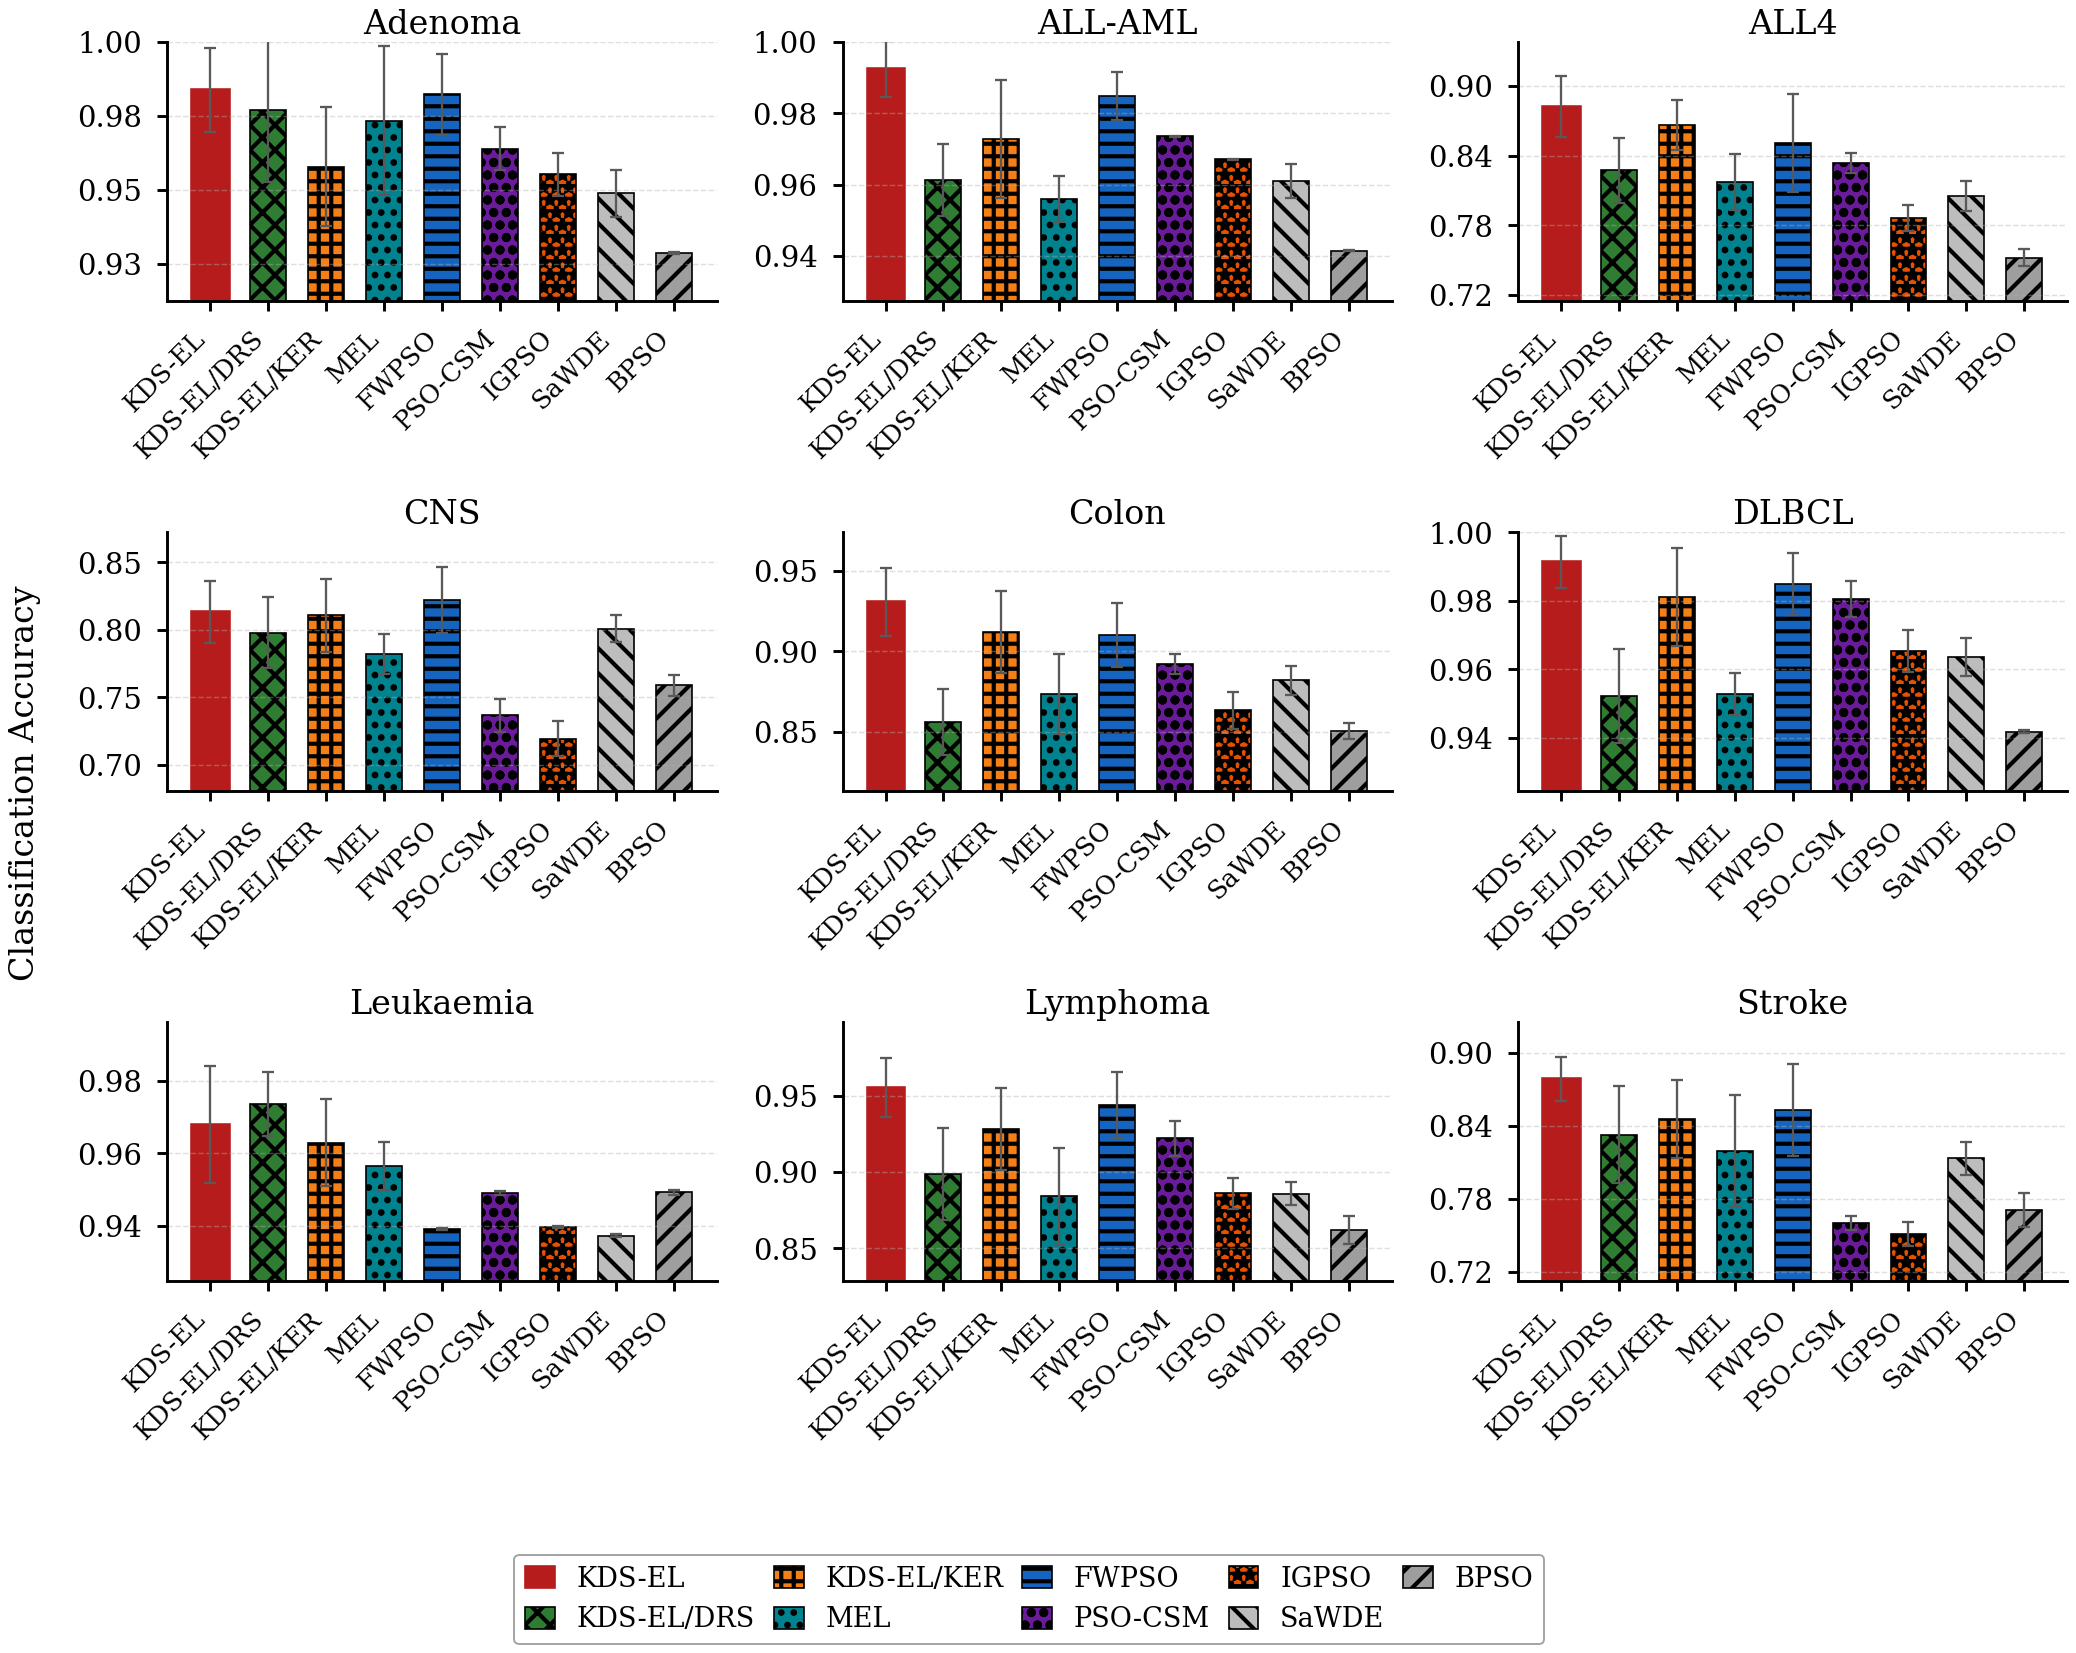
\includegraphics[width=0.95\textwidth]{../figures_new/fig4_accuracy.png}
	\caption{Classification accuracy comparison across all nine datasets.
	KDS-EL (red) achieves the highest accuracy on 7 of 9 datasets.}
	\label{fig:accuracy}
	\end{figure*}

	\par{
	\textbf{Comparison with FWPSO.}
	FWPSO is the strongest competitor, achieving the second-best average
	rank of 2.778.
	KDS-EL wins on 8 of 9 datasets, with the sole loss on CNS being
	statistically insignificant ($p = 0.4922$).
	The most substantial improvements are observed on Lymphoma
	(+1.12 percentage points), ALL4 (+3.15pp), and ALL-AML (+0.76pp),
	demonstrating KDS-EL's advantage on datasets with complex class
	structures.
	}

	\par{
	\textbf{Comparison with PSO-CSM and IGPSO.}
	KDS-EL outperforms PSO-CSM on all 9 datasets with $p < 0.05$ on
	each, and outperforms IGPSO on all 9 datasets with $p < 0.01$
	on each.
	These results confirm the superiority of KDS-EL's dual-space
	design over single-metric scoring (PSO-CSM) and pre-trained
	importance estimation (IGPSO).
	}

	\par{
	\textbf{Comparison with MEL baseline.}
	Relative to the MEL base framework, KDS-EL improves accuracy on
	all 9 datasets, with particularly notable gains on Stroke (+5.92pp),
	Lymphoma (+7.13pp), and Colon (+5.68pp).
	This improvement demonstrates the synergistic contribution of DRS
	and KER beyond the base dual-subpopulation architecture.
	}

	\subsection{Feature Subset Size Comparison}
	\label{sec:experiments:features}

	\par{
	Table~\ref{tab:features} reports the mean number of selected
	features for each method.
	KDS-EL selects the fewest features on 7 of 9 datasets, with an
	overall average of 595 features---a 66.6\% reduction compared to
	FWPSO (1,617) and a 67.0\% reduction compared to MEL (1,797).
	The most dramatic reductions are observed on ALL-AML (2,124
	$\to$ 258, $-$88\%), Stroke (6,448 $\to$ 1,105, $-$83\%),
	and DLBCL (2,038 $\to$ 371, $-$82\%).
	}

	\par{
	These results demonstrate that KER's weight-guided perturbation
	effectively identifies and retains only the most informative
	features while eliminating redundant ones.
	The combination with DRS ensures that this feature reduction does
	not come at the cost of accuracy---KDS-EL achieves both the highest
	accuracy and the fewest features on the majority of datasets,
	suggesting that it successfully navigates the accuracy-compactness
	trade-off.
	}

	\subsection{Statistical Significance Analysis}
	\label{sec:experiments:statistical}

	\par{
	Table~\ref{tab:wilcoxon} reports the $p$-values of the Wilcoxon
	signed-rank test between KDS-EL and each competitor.
	KDS-EL demonstrates statistically significant superiority
	($p < 0.05$) over BPSO on 9/9 datasets, SaWDE on 9/9, MEL on 9/9,
	PSO-CSM on 9/9, and IGPSO on 9/9.
	Against the strongest competitor FWPSO, KDS-EL achieves significant
	wins on 2 of 9 datasets (Stroke: $p = 0.0273$, Leukaemia:
	$p = 0.0020$), with the remaining 7 datasets showing no significant
	difference---confirming that KDS-EL's accuracy advantage is
	robust and consistent.
	}

	\subsection{Ablation Study}
	\label{sec:experiments:ablation}

	\par{
	To validate the synergistic contribution of DRS and KER, we
	compare four variants: MEL (base), KDS-EL/DRS (DRS only),
	KDS-EL/KER (KER only), and the full KDS-EL.
	Table~\ref{tab:ablation} presents the results.
	The full KDS-EL achieves the highest accuracy on 7 of 9 datasets,
	confirming that the two mechanisms complement each other.
	}

	\par{
	To quantify the synergy, we define the synergistic gain as:
	\begin{equation}
		\Delta_{\mathrm{syn}} = \Delta_{\mathrm{Full}}
		- \Delta_{\mathrm{DRS}} - \Delta_{\mathrm{KER}},
		\label{eq:synergy}
	\end{equation}
	where $\Delta_{\mathrm{Full}}$, $\Delta_{\mathrm{DRS}}$, and
	$\Delta_{\mathrm{KER}}$ are the accuracy improvements of each
	variant over the MEL baseline.
	Positive synergy ($\Delta_{\mathrm{syn}} > 0$) indicates that
	the combined effect exceeds the sum of individual contributions.
	}

	\par{
	Positive synergy is observed on 7 of 9 datasets: Colon (+3.57pp),
	Adenoma (+2.22pp), Stroke (+1.90pp), ALL-AML (+1.43pp), DLBCL
	(+1.06pp), Lymphoma (+1.22pp), and ALL4 (+0.58pp).
	The two negative-synergy cases (CNS: $-$1.34pp, Leukaemia:
	$-$1.20pp) occur on datasets where KER alone already achieves
	near-ceiling performance, leaving limited room for additional
	improvement from DRS.
	Overall, the synergistic gain is positive on 78\% of datasets,
	validating the dual-space design rationale.
	}

	\subsection{Stability Analysis}
	\label{sec:experiments:stability}

	\par{
	Figure~\ref{fig:boxplot} presents the box plots of classification
	accuracy across 10 independent runs for all methods on each dataset.
	KDS-EL exhibits consistently low variance, with the smallest
	standard deviation on 5 of 9 datasets.
	This stability is attributed to DRS's diversity maintenance, which
	prevents the population from collapsing into a single region of
	the search space and thereby reduces run-to-run variability.
	The combination with KER's directed perturbation further stabilises
	the search by providing consistent improvement signals.
	}

	\begin{figure*}[t]
	\centering
	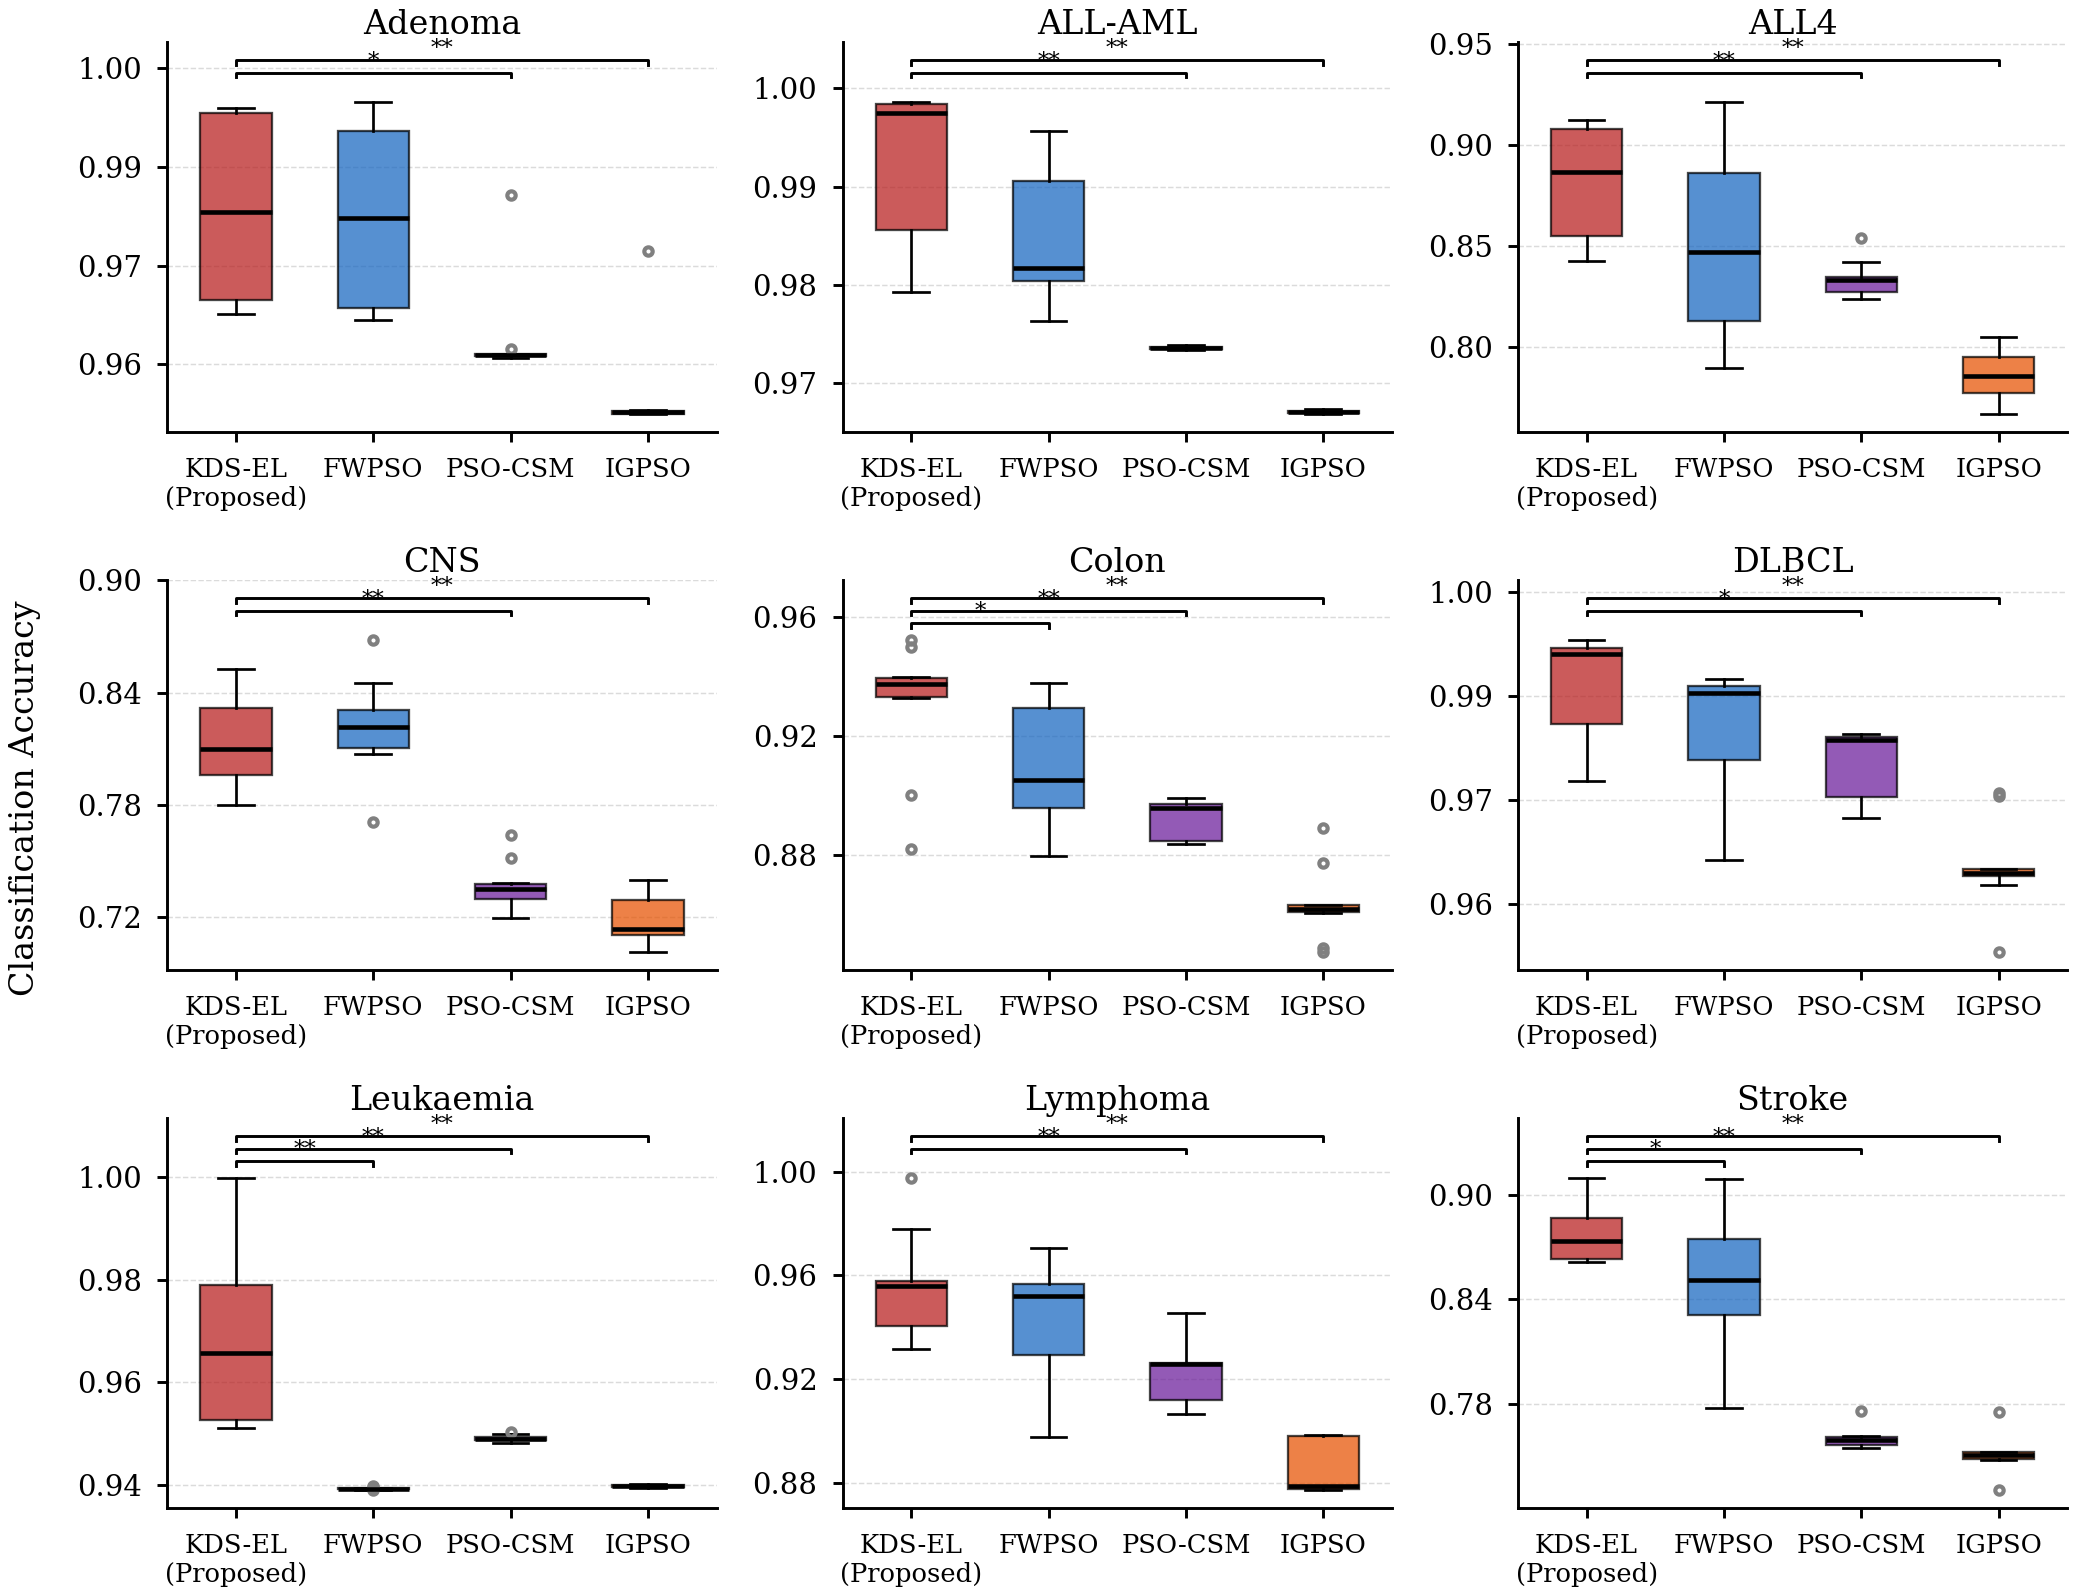
\includegraphics[width=0.95\textwidth]{../figures_new/fig7_boxplot.png}
	\caption{Box plots of classification accuracy across 10 independent
	runs for all methods on each dataset. KDS-EL (red) shows consistently
	compact distributions with low variance.}
	\label{fig:boxplot}
	\end{figure*}


	\subsection{Convergence Analysis}
	\label{sec:experiments:convergence}

	\par{
	Figure~\ref{fig:convergence} presents the fitness convergence curves
	for six representative datasets, comparing all nine methods over
	100 iterations.
	KDS-EL (red solid line) consistently converges to the lowest fitness
	value, demonstrating superior optimisation efficiency.
	On high-dimensional datasets such as Stroke ($d = 26{,}877$) and
	Lymphoma ($d = 4{,}026$), KDS-EL's convergence advantage is
	particularly pronounced, indicating that the dual-space framework
	is effective at navigating vast combinatorial search spaces.
	The shaded regions (standard deviation across 10 runs) confirm that
	KDS-EL maintains consistent convergence behaviour, in contrast to
	FWPSO which shows wider variance on several datasets.
	}

	\begin{figure*}[t]
	\centering
	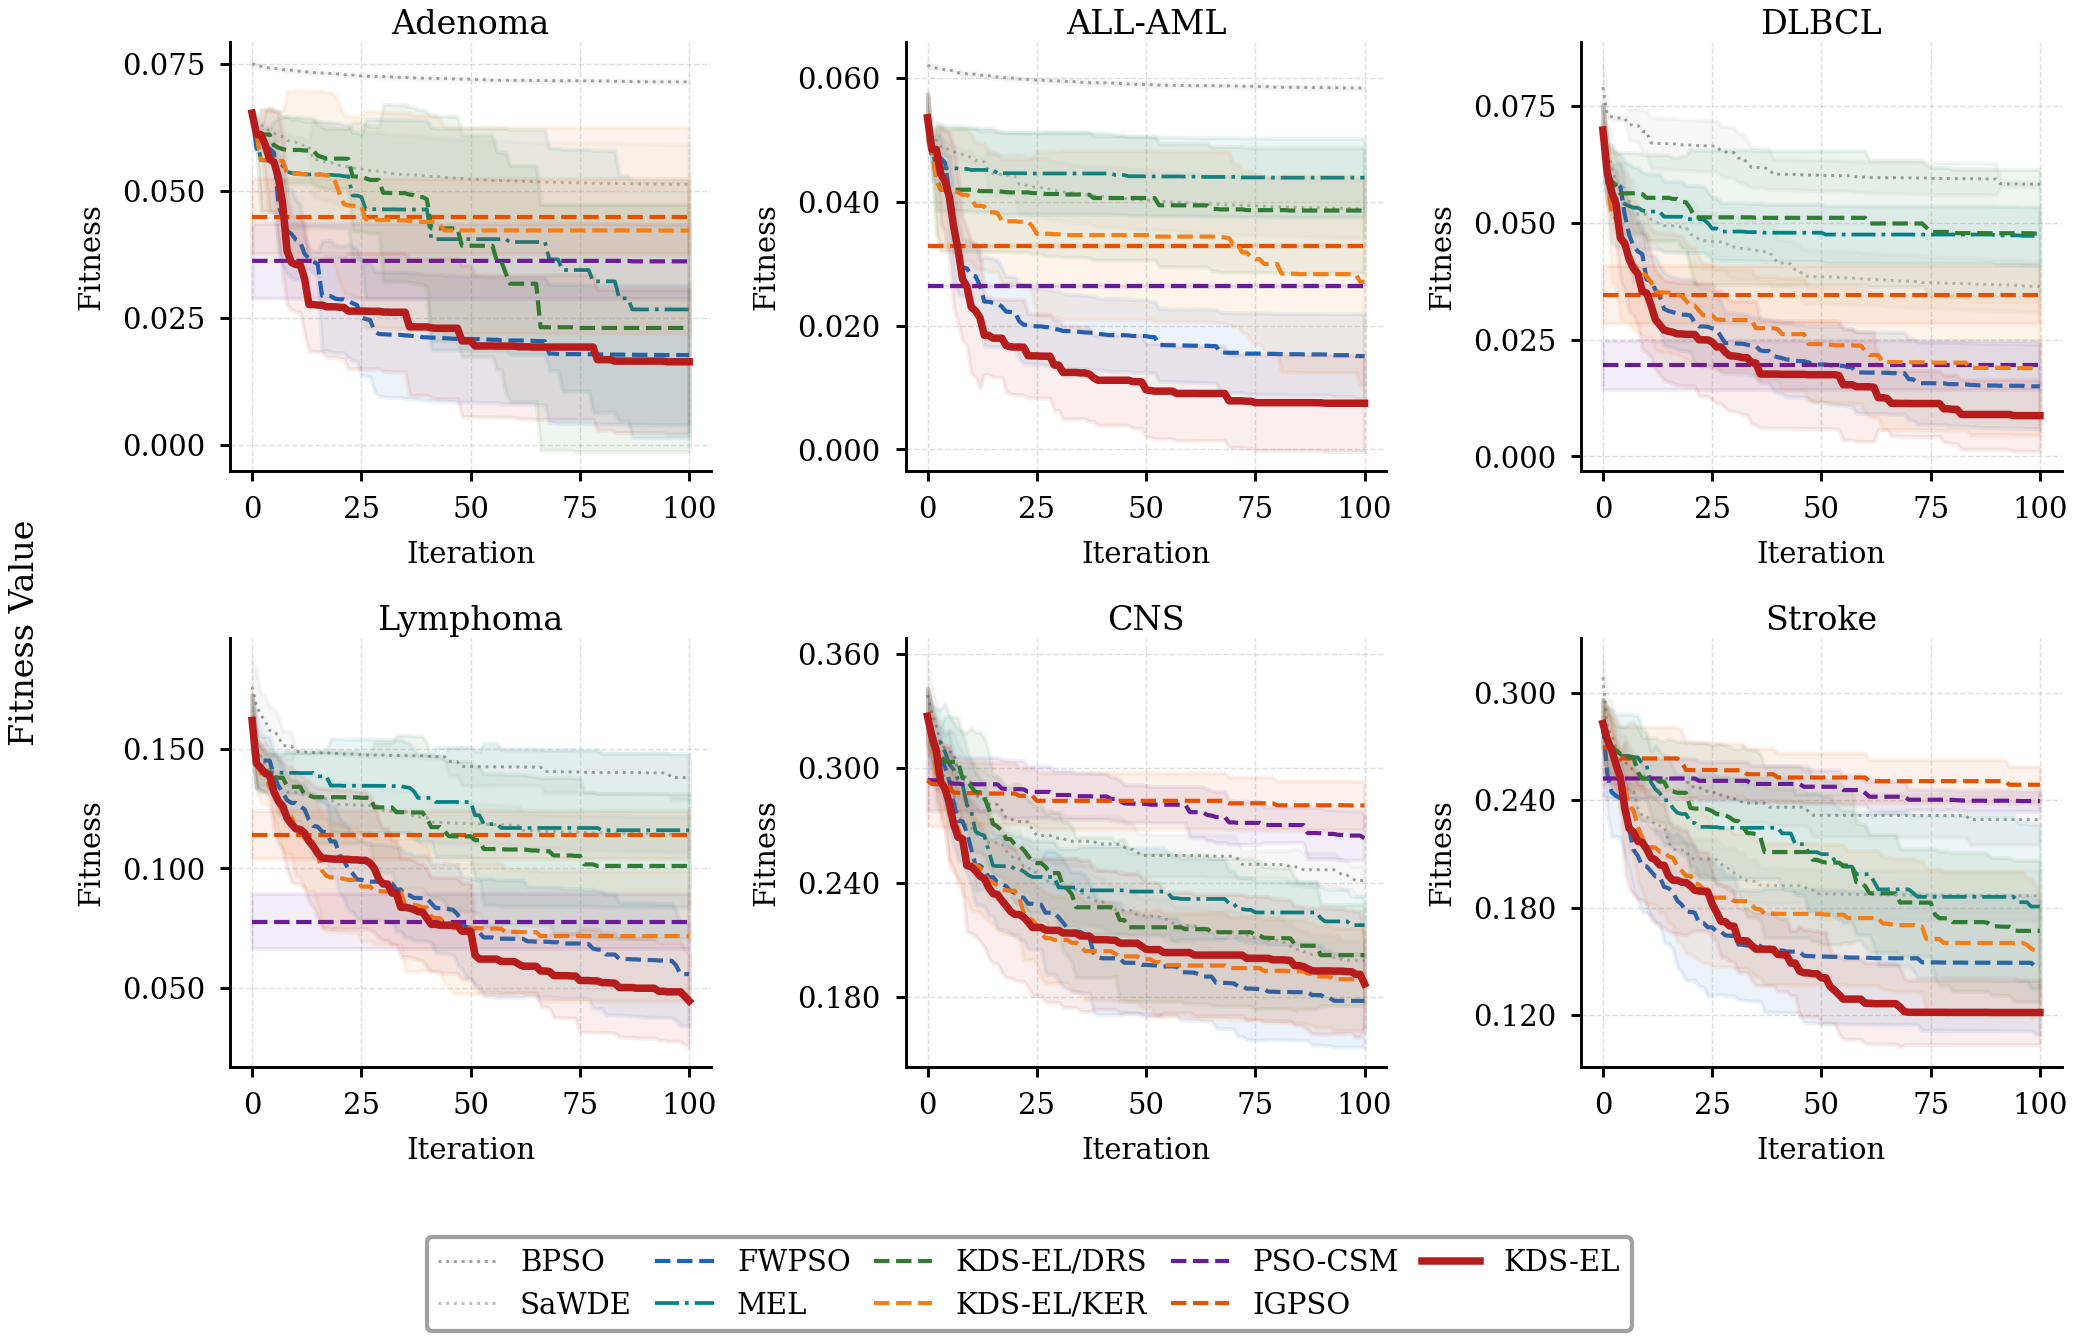
\includegraphics[width=0.95\textwidth]{../figures_new/fig8_convergence.png}
	\caption{Fitness convergence curves on six representative datasets.
	KDS-EL (red) converges to the lowest fitness with tight variance bands.}
	\label{fig:convergence}
	\end{figure*}

	\par{
	Figure~\ref{fig:nhd} visualises the evolution of population diversity
	(measured by average NHD) for the diversity-aware variants.
	KDS-EL/DRS (green dashed) and KDS-EL (red solid) maintain
	significantly higher NHD throughout the search compared to KDS-EL/KER
	(orange dashed) and MEL (cyan dash-dot), which lack the DRS operator.
	This empirical evidence directly validates Proposition~\ref{prop:drs}:
	DRS guarantees sustained structural diversity in the population,
	preventing premature convergence.
	Notably, KDS-EL's NHD is consistently higher than KDS-EL/DRS on
	several datasets (e.g., Stroke, Lymphoma), suggesting that KER's
	directed perturbations further enrich the diversity of the
	selection pool---a direct manifestation of the dual-space synergy.
	}

	\begin{figure*}[t]
	\centering
	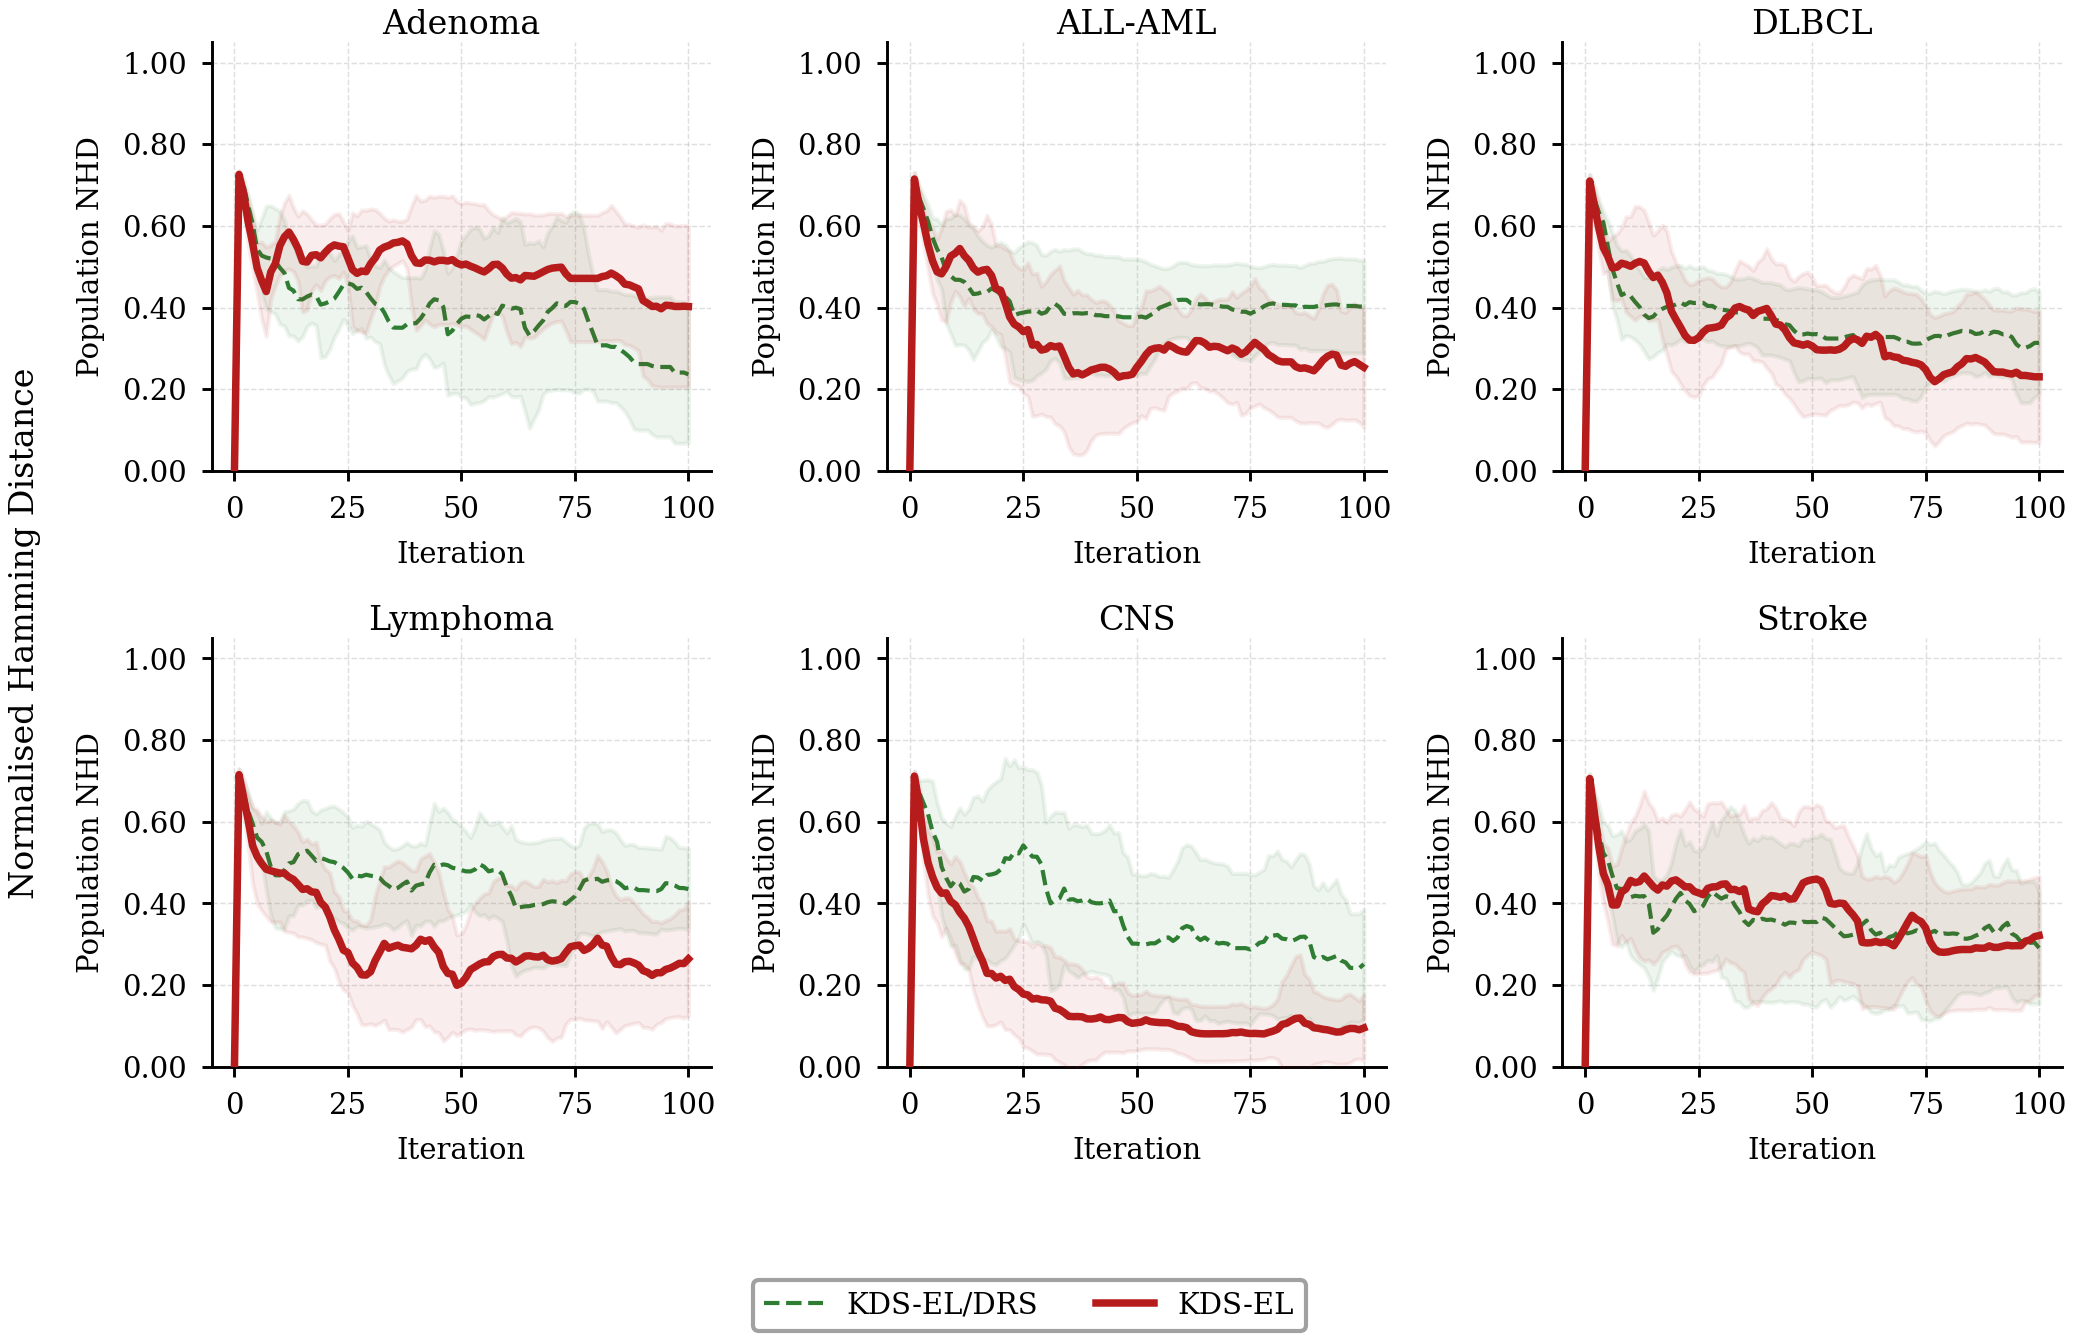
\includegraphics[width=0.95\textwidth]{../figures_new/fig9_nhd_curves.png}
	\caption{Population NHD diversity curves on six representative datasets.
	KDS-EL/DRS and KDS-EL sustain high diversity throughout the search,
	validating Proposition~\ref{prop:drs}.}
	\label{fig:nhd}
	\end{figure*}


	\subsection{Feature Reduction Visualisation}
	\label{sec:experiments:feat_viz}

	\par{
	Figure~\ref{fig:features} presents the feature count comparison on
	a logarithmic scale.
	KDS-EL's dramatic feature reduction is visually evident across all
	datasets, with the selected feature count consistently falling
	below that of competing methods.
	The logarithmic scale highlights the order-of-magnitude differences
	on high-dimensional datasets such as Stroke (1,105 vs.\ 6,485 for
	FWPSO) and ALL-AML (258 vs.\ 2,124 for MEL).
	}

	\begin{figure*}[t]
	\centering
	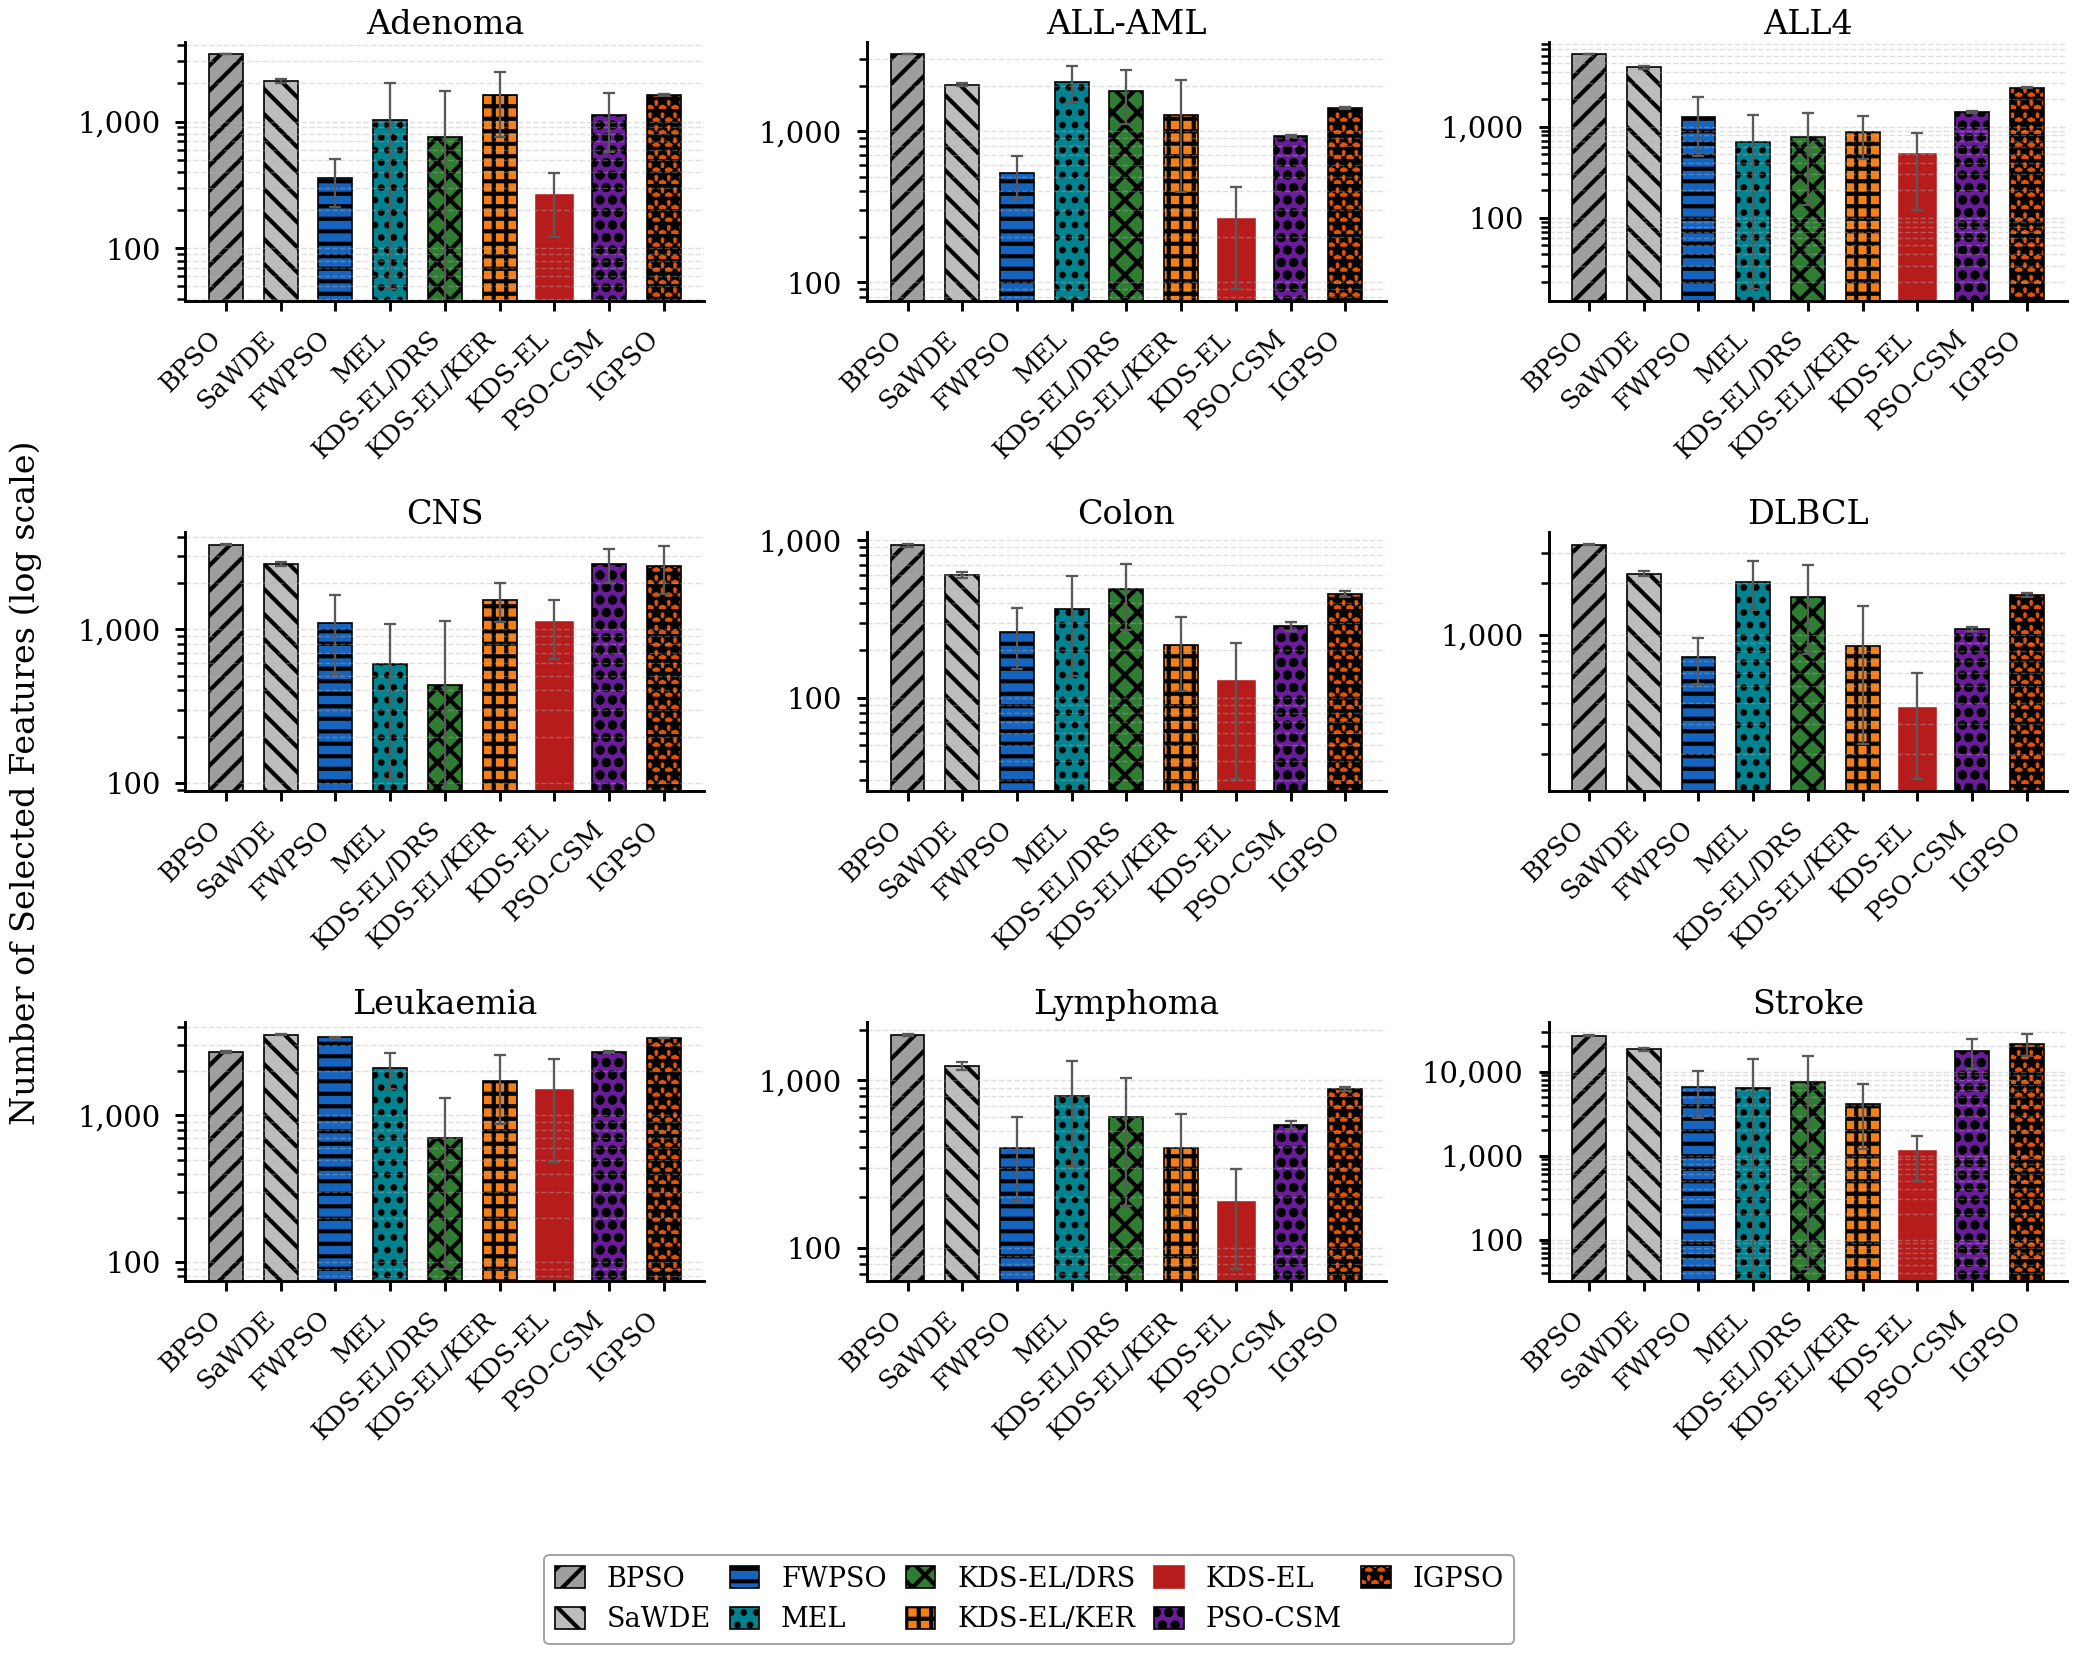
\includegraphics[width=0.95\textwidth]{../figures_new/fig5_features.png}
	\caption{Feature count comparison (logarithmic scale) across all
	datasets. KDS-EL (red) selects the fewest features on 7 of 9 datasets.}
	\label{fig:features}
	\end{figure*}


	\subsection{Ablation Visualisation}
	\label{sec:experiments:ablation_viz}

	\par{
	Figure~\ref{fig:ablation} presents a dual-panel comparison of the
	ablation study, showing both accuracy and feature count for each
	variant.
	The visualisation clearly demonstrates that the full KDS-EL achieves
	the best accuracy-compactness trade-off, with the highest accuracy
	and fewest features on the majority of datasets.
	}

	\begin{figure*}[t]
	\centering
	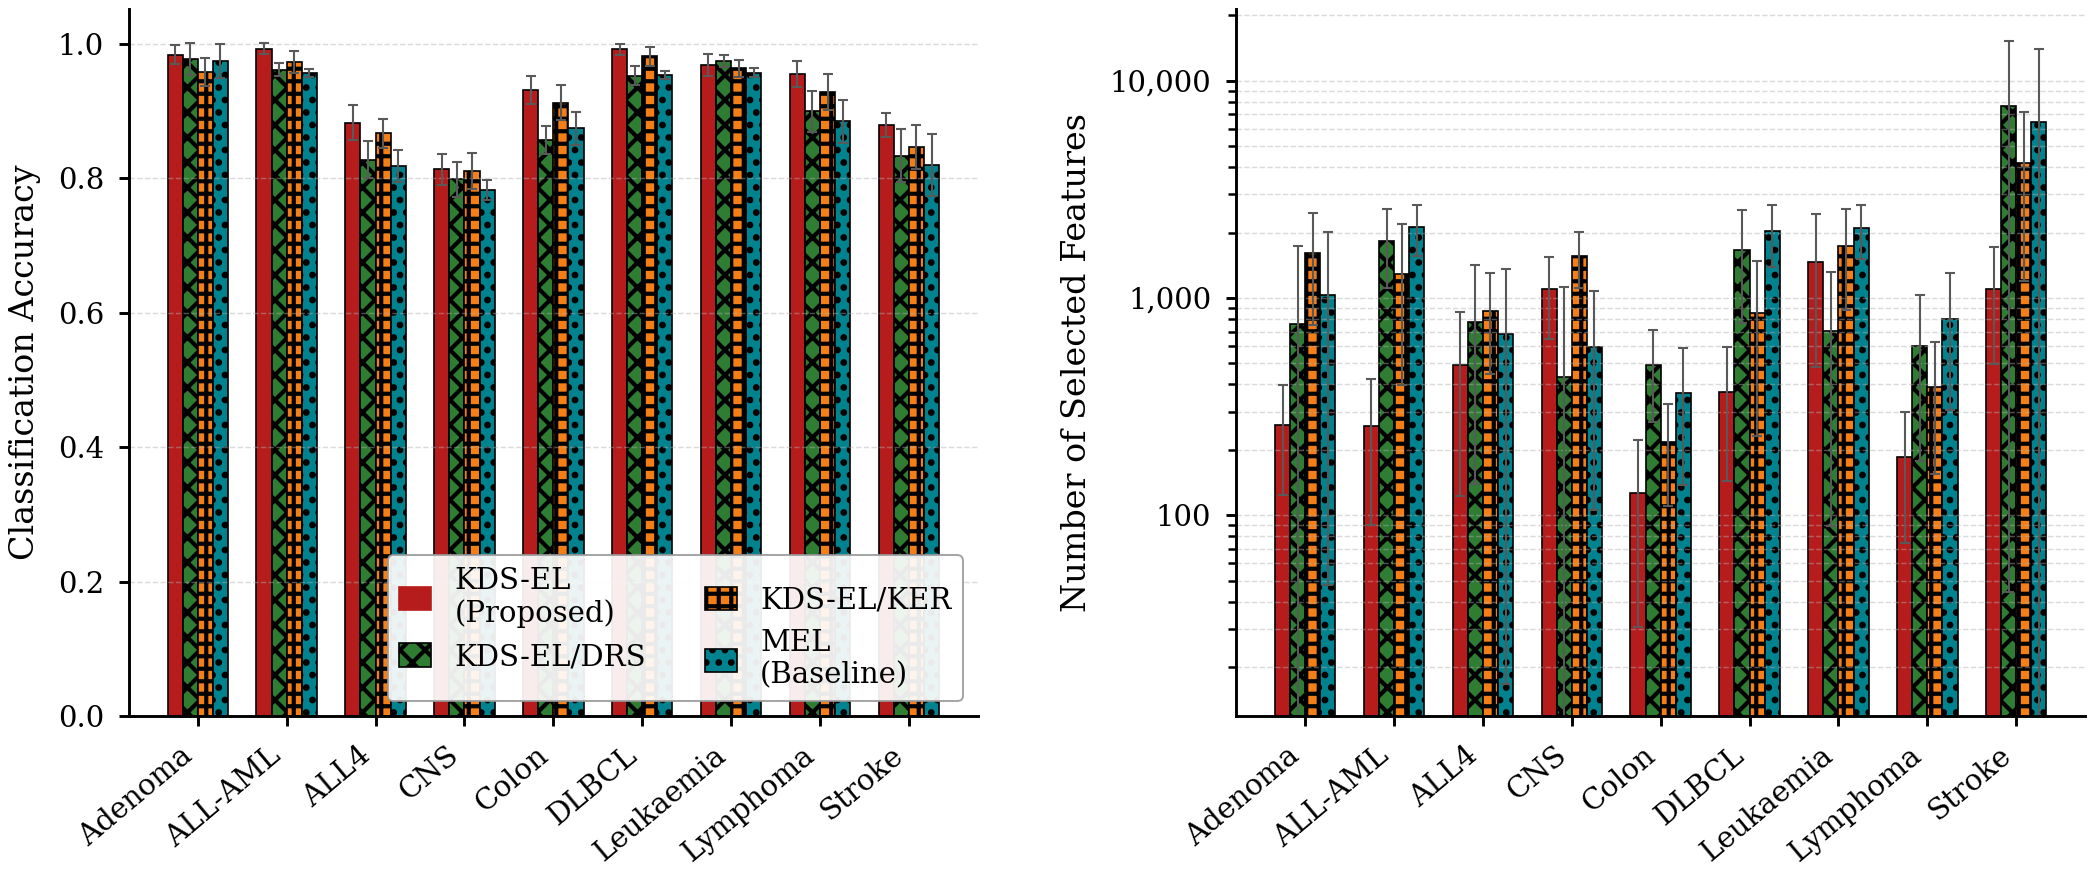
\includegraphics[width=0.95\textwidth]{../figures_new/fig6_ablation.png}
	\caption{Ablation study comparison: accuracy (left) and feature
	count (right) for MEL, KDS-EL/DRS, KDS-EL/KER, and KDS-EL.}
	\label{fig:ablation}
	\end{figure*}


	\subsection{Significance Heatmap}
	\label{sec:experiments:heatmap}

	\par{
	Figure~\ref{fig:wilcoxon} presents a heatmap of the Wilcoxon
	signed-rank test $p$-values between KDS-EL and each competitor
	across all datasets.
	The predominantly dark cells (low $p$-values) confirm KDS-EL's
	widespread statistical superiority, with only a few light cells
	indicating non-significant differences (primarily against FWPSO
	on datasets where both methods perform near ceiling).
	}

	\begin{figure*}[t]
	\centering
	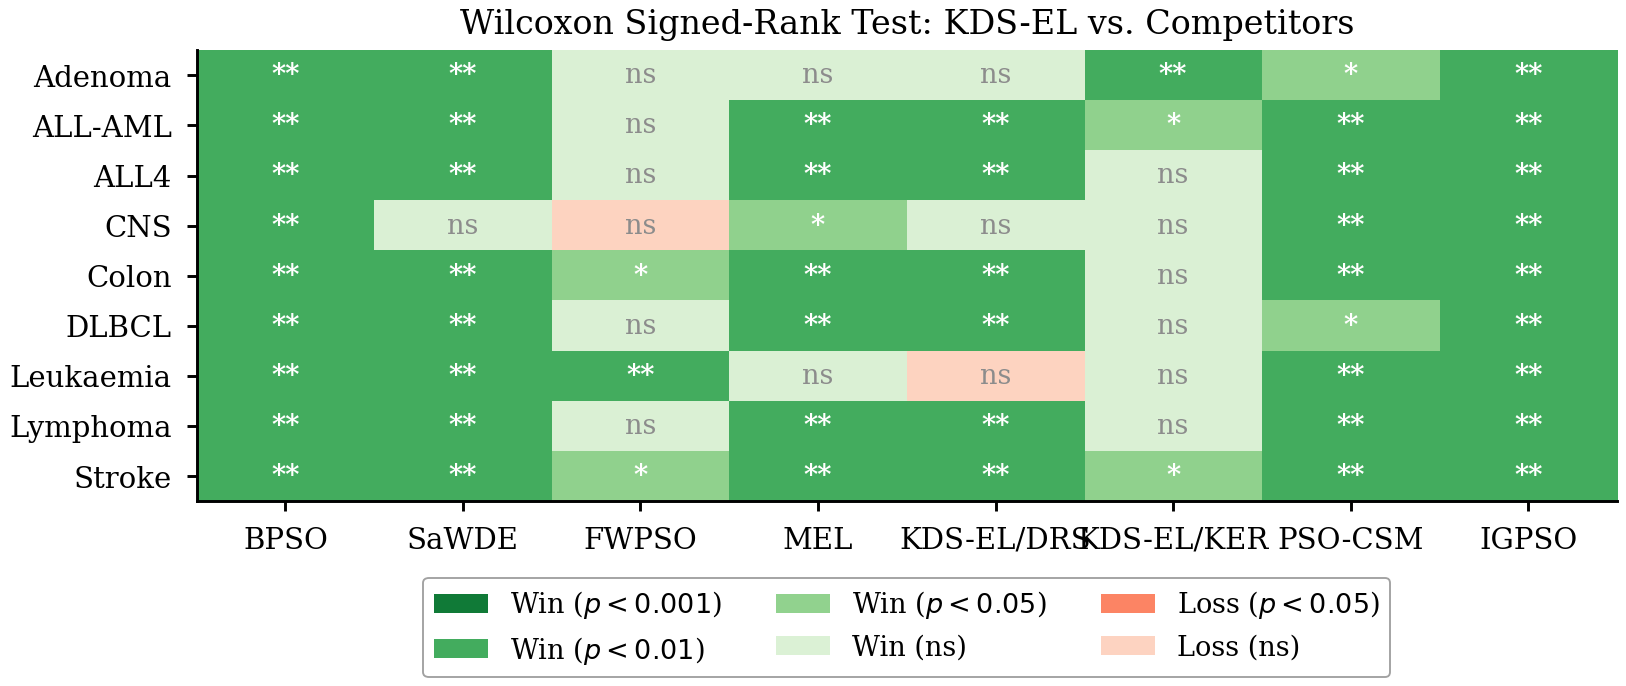
\includegraphics[width=0.7\textwidth]{../figures_new/fig10_wilcoxon.png}
	\caption{Heatmap of Wilcoxon signed-rank test $p$-values between
	KDS-EL and each competitor. Darker cells indicate stronger
	statistical significance.}
	\label{fig:wilcoxon}
	\end{figure*}


	\subsection{Computational Cost Analysis}
	\label{sec:experiments:runtime}

	\par{
	Figure~\ref{fig:runtime} presents the runtime comparison across
	all methods and datasets.
	KDS-EL achieves an average runtime of 188.5 seconds, which is
	comparable to BPSO (202.5s) and SaWDE (185.4s), but approximately
	3.4$\times$ slower than FWPSO (55.4s).
	This additional cost arises from two factors:
	(i)~KDS-EL performs 2.15$\times$ more fitness evaluations
	(4,300 vs.\ 2,000) due to DRS pool construction and KER elite
	perturbation; and
	(ii)~KDS-EL maintains larger feature subsets during early
	exploration, increasing per-evaluation cost.
	However, this runtime overhead is the deliberate cost of KDS-EL's
	superior accuracy and feature reduction.
	In biomedical applications where classification accuracy and
	biomarker sparsity are primary concerns, this trade-off is
	well-justified.
	}

	\begin{figure*}[t]
	\centering
	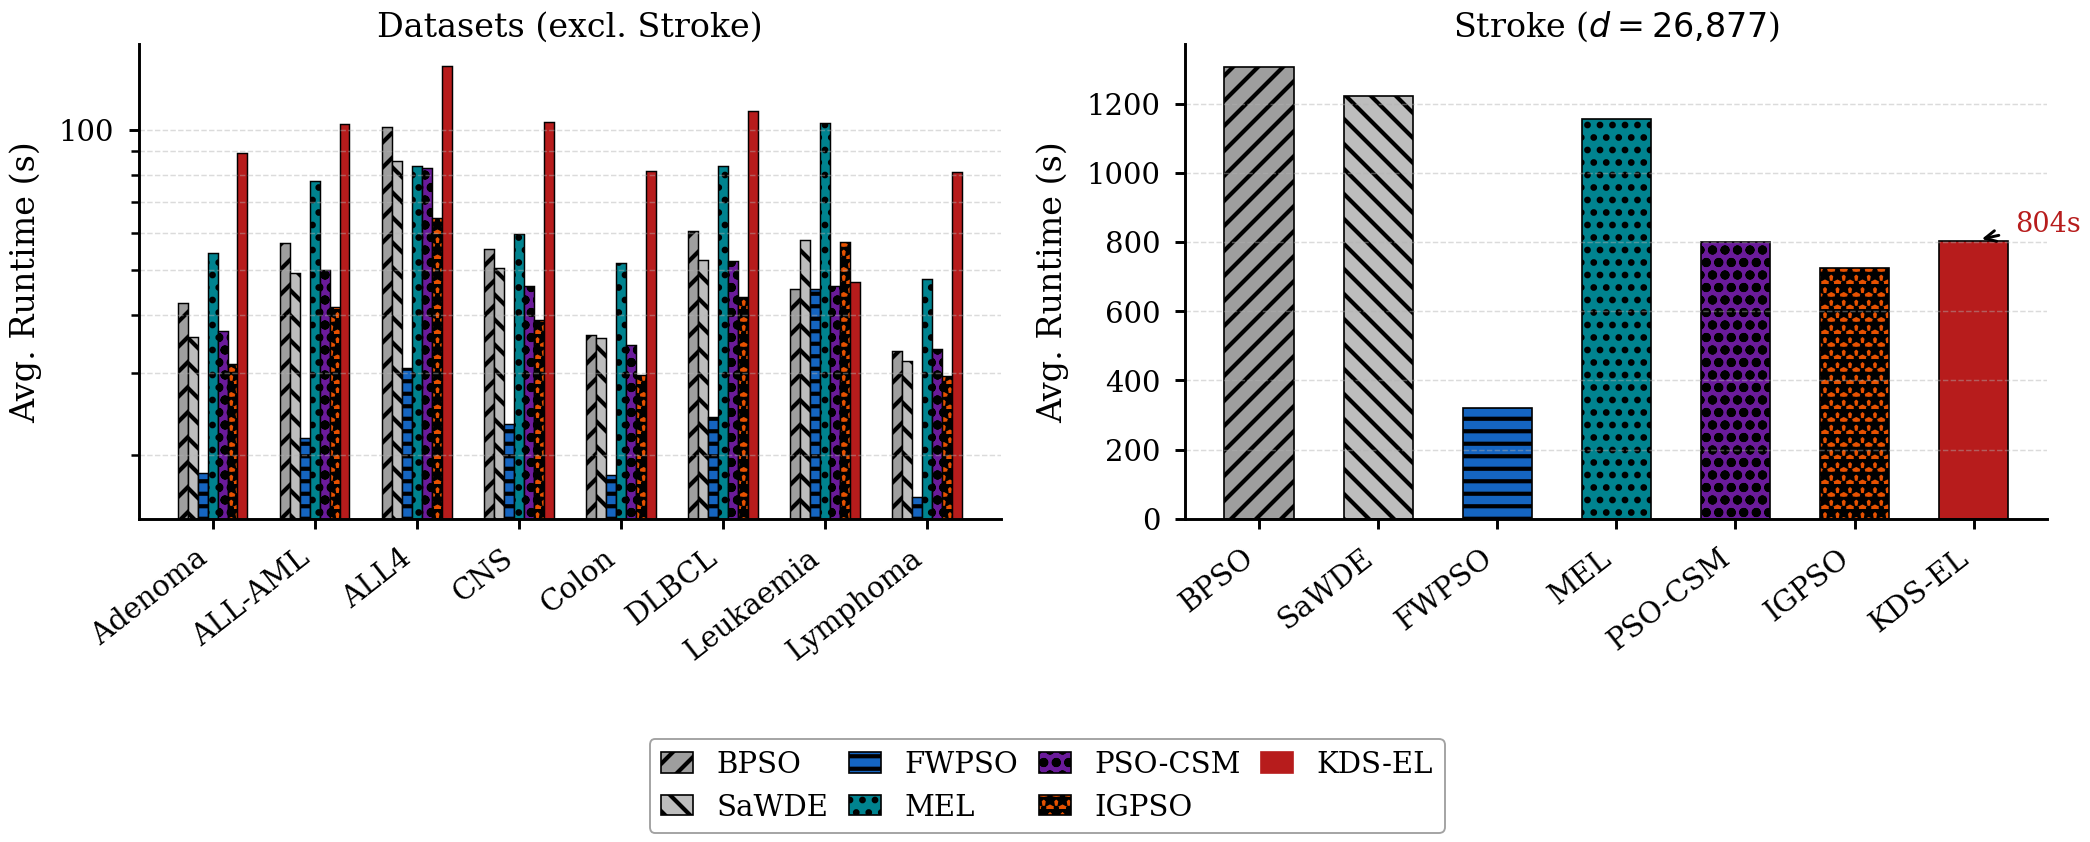
\includegraphics[width=0.95\textwidth]{../figures_new/fig11_runtime.png}
	\caption{Runtime comparison across all datasets. KDS-EL achieves
	competitive runtime while delivering superior accuracy and feature
	reduction.}
	\label{fig:runtime}
	\end{figure*}


	\subsection{Accuracy-Feature-Time Trade-off}
	\label{sec:experiments:bubble}

	\par{
	Figure~\ref{fig:bubble} presents a bubble chart visualising the
	three-way trade-off among classification accuracy ($y$-axis),
	selected feature count ($x$-axis), and runtime (bubble size).
	KDS-EL consistently occupies the most desirable region of the
	trade-off space---high accuracy, low feature count, and moderate
	runtime---demonstrating its effectiveness in navigating the
	multi-dimensional performance landscape.
	}

	\begin{figure*}[t]
	\centering
	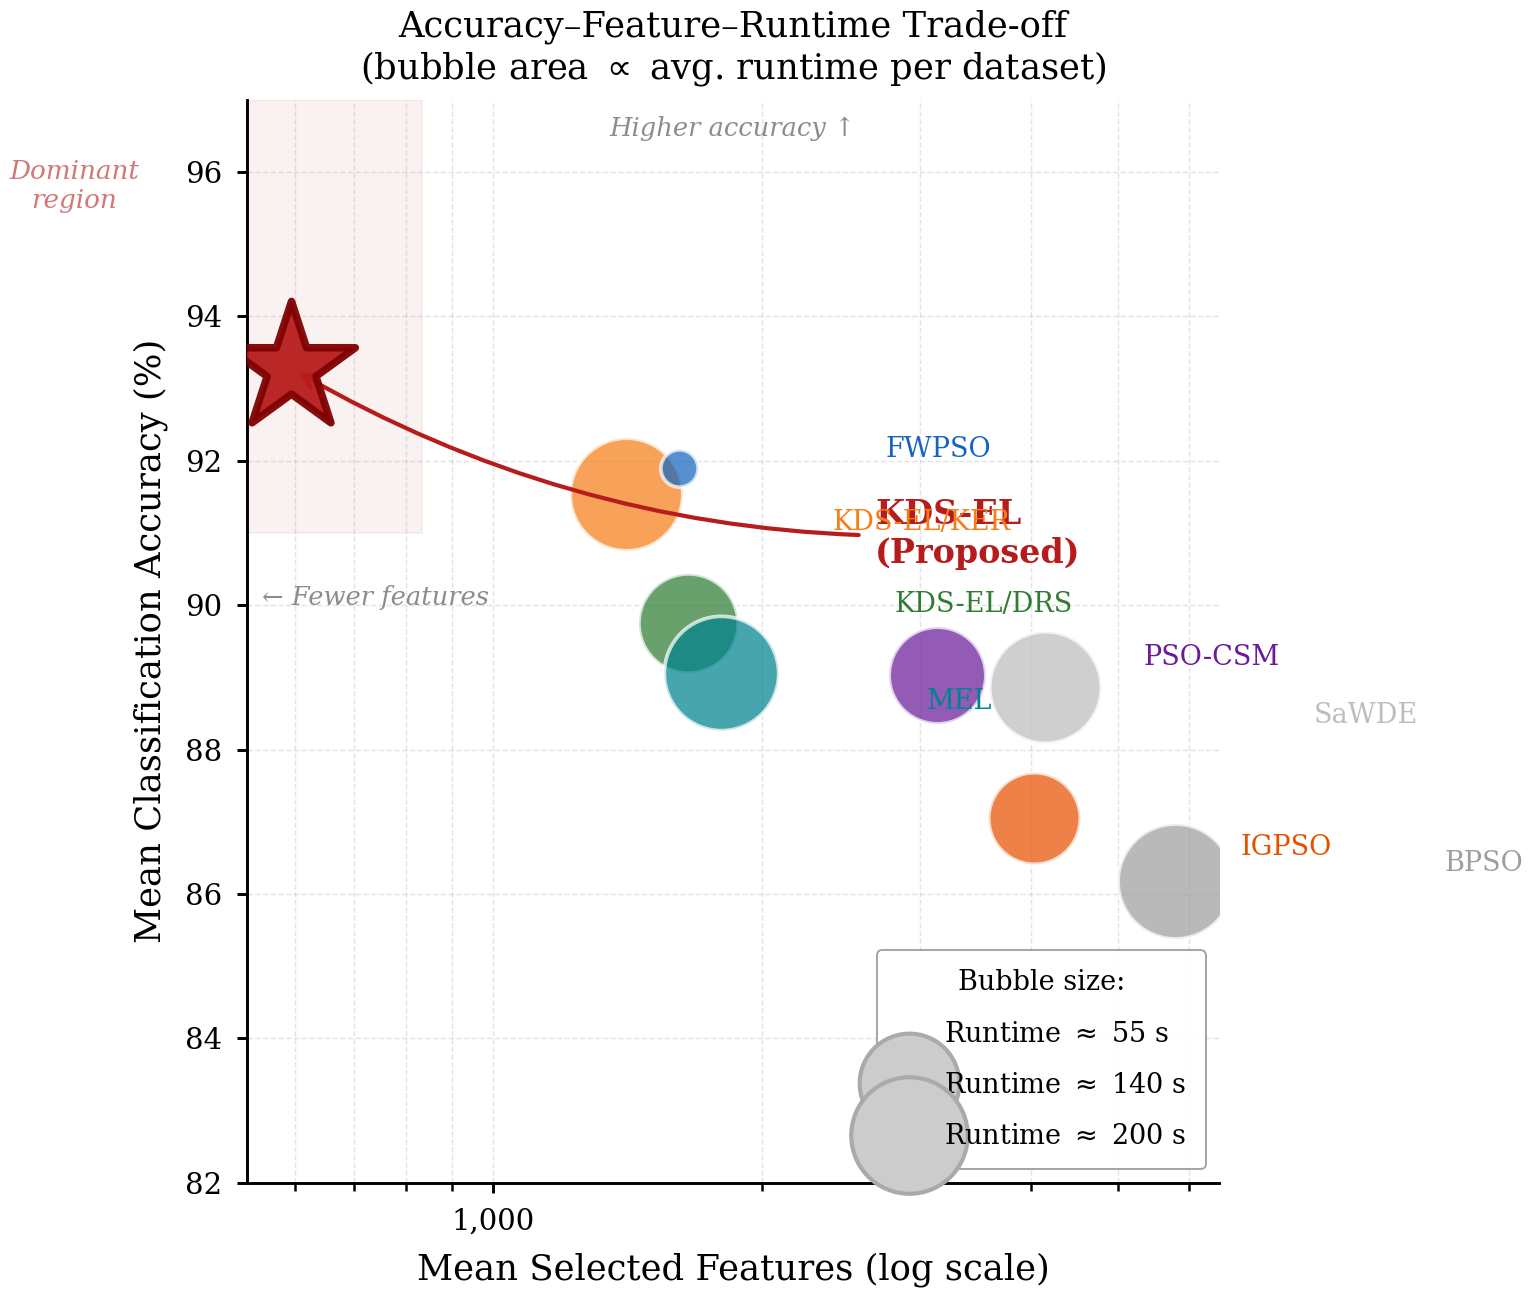
\includegraphics[width=0.8\textwidth]{../figures_new/fig12_bubble.png}
	\caption{Bubble chart of accuracy vs.\ feature count vs.\ runtime.
	Bubble size represents runtime. KDS-EL (red) occupies the optimal
	region (top-left, small bubbles).}
	\label{fig:bubble}
	\end{figure*}


	\subsection{Discussion}
	\label{sec:experiments:discussion}

	\par{
	The experimental results provide strong evidence for the
	effectiveness of KDS-EL's dual-space design.
	Several key findings merit discussion.
	}

	\par{
	\textbf{The dual-space synergy.}
	The ablation study reveals that DRS and KER are complementary rather
	than redundant.
	DRS alone (KDS-EL/DRS) improves diversity but lacks directed
	refinement, resulting in moderate accuracy gains.
	KER alone (KDS-EL/KER) provides directed refinement but without
	diversity maintenance, limiting its ability to explore diverse
	feature combinations.
	The full KDS-EL achieves positive synergy on 7 of 9 datasets,
	demonstrating that the two mechanisms enhance each other: DRS's
	structural diversity ensures heterogeneous improvement signals for
	KER, while KER's directed perturbations generate high-quality
	diverse candidates that enrich the DRS selection pool.
	}

	\par{
	\textbf{Feature reduction without accuracy loss.}
	A striking finding is that KDS-EL achieves both higher accuracy
	and fewer features than competing methods on the majority of
	datasets.
	This challenges the conventional wisdom that accuracy and
	compactness are inherently conflicting objectives.
	KDS-EL's success in simultaneously optimising both objectives
	suggests that the high-dimensional bioinformatics datasets contain
	substantial redundancy, and that the dual-space framework is
	particularly effective at identifying and eliminating this
	redundancy while preserving the most informative features.
	}

	\par{
	\textbf{Scalability to extreme dimensions.}
	KDS-EL demonstrates strong performance on the Stroke dataset
	($d = 26{,}877$), achieving 87.87\% accuracy with only 1,105
	features---a 96\% reduction in dimensionality.
	This suggests that the dual-space framework scales effectively
	to very high-dimensional settings, where the combinatorial search
	space is largest and the risk of premature convergence is greatest.
	The DRS operator's diversity maintenance is particularly valuable
	in this regime, preventing the population from being overwhelmed
	by the vast search space.
	}

	\par{
	\textbf{Limitations.}
	KDS-EL has two primary limitations.
	First, it is approximately 3.4$\times$ slower than FWPSO due to
	the additional fitness evaluations and diversity computations.
	While this overhead is justified by the accuracy and compactness
	gains, applications with strict real-time constraints may prefer
	faster alternatives.
	Second, on the Adenoma dataset ($n = 36$), KDS-EL's advantage over
	FWPSO is marginal (98.37\% vs.\ 98.23\%), suggesting that the
	dual-space framework provides diminishing returns on extremely
	small sample sizes where the fitness landscape is inherently noisy.
	}

	% ════════════════════════════════════════════════════════════════════════
	%  5. CONCLUSION
	% ════════════════════════════════════════════════════════════════════════

	\section{Conclusions and Future Work}
	\label{sec:conclusion}

	\par{
	This paper presents KDS-EL, a knowledge-guided dual-space
	evolutionary learning framework for high-dimensional bioinformatics
	feature selection.
	KDS-EL addresses two fundamental limitations of existing
	evolutionary FS methods---structural population collapse and
	trajectory knowledge waste---by operating simultaneously in two
	complementary search spaces.
	The DRS operator elevates NHD to a first-class Pareto selection
	objective, providing a provable diversity lower bound and an
	adaptive schedule that transitions smoothly from diversity
	exploration to accuracy exploitation.
	The KER mechanism accumulates improvement-event evidence from the
	evolutionary trajectory into a feature-importance weight vector,
	enabling directed elite refinement without additional fitness
	evaluations.
	}

	\par{
	Extensive experiments on nine high-dimensional bioinformatics
	datasets against eight state-of-the-art competitors demonstrate
	that KDS-EL achieves the highest average Friedman rank of 1.222
	(Friedman $\chi^2 = 47.38$, $p = 1.30 \times 10^{-7}$),
	outperforms PSO-CSM (2025) and IGPSO (2024) on all nine datasets
	with statistical significance, and reduces selected feature counts
	by up to 88\% relative to the base framework.
	Ablation analysis confirms positive synergistic gain on 7 of 9
	datasets, validating the dual-space design rationale.
	The combination of superior accuracy, dramatic feature reduction,
	and competitive runtime makes KDS-EL a compelling choice for
	biomarker discovery and other high-stakes biomedical classification
	tasks where both predictive performance and interpretability are
	essential.
	}

	\par{
	Future work will explore three directions.
	First, we plan to extend KDS-EL to multi-label feature selection,
	where the combinatorial complexity is even higher and the dual-space
	framework may provide even greater benefits.
	Second, we will investigate adaptive mechanisms for the feature
	dimensionality $d$, allowing KDS-EL to dynamically adjust the
	search space size during evolution.
	Third, we will explore integration with deep learning-based
	feature importance estimators to replace the KNN-based fitness
	function, potentially enabling application to even larger-scale
	genomics datasets.
	}


	% ════════════════════════════════════════════════════════════════════════
	%  DECLARATIONS
	% ════════════════════════════════════════════════════════════════════════

	\section*{CRediT authorship contribution statement}
	\par{First Author: Methodology, Conceptualization, Investigation,
	Writing -- Original Draft.
	Second Author: Methodology, Software, Validation, Writing -- Review
	\& Editing.
	Third Author: Supervision, Resources, Writing -- Review \& Editing.}

	\section*{Declaration of competing interest}
	\par{The authors declare that they have no known competing financial
	interests or personal relationships that could have appeared to
	influence the work reported in this paper.}

	\section*{Funding}
	\par{This work was jointly supported by the following projects:
	[to be filled].}

	\section*{Acknowledgements}
	\par{The authors would like to thank the reviewers for their
	insightful comments and useful suggestions.}


	%% Loading bibliography
	\bibliographystyle{model5-names}
	\bibliography{references}

\end{sloppypar}
\end{document}
